%=========================================================================
% (c) Michal Bidlo, Bohuslav Křena, 2008

\iffalse

Způsoby, jak reprezentovat a uchovávat \emph{entity} existuje velké množství. V začátcích herního průmyslu byly \emph{entity} velmi úzce provázány s okolním kódem, ale díky velikosti týmů, které na hrách pracovaly, a relativní jednoduchosti her toto nebyl problém. Avšak s růstem složitosti se začaly používat další přístupy, jako například \emph{objektově orientované programování}, kdy je využíván \emph{polymorfismus} a \emph{dědičnost}. 

Cílem této práce je návrh a implementace knihovny pro dynamickou kompozici objektů, za běhu aplikace. Mezi hlavní požadavky patří \emph{thread-safe}\cite{ThreadSafety} rozhraní, které je možné používat ve vícevláknových aplikacích. Další prioritou je skutečné využití a prospěch z běhu na více vláknech, jednoduchost použití a integrace do již existujících projektů a minimalizace režie.

Práce je rozdělena do čtyř logických celků -- teoretická část\ref{Chap:Theory}, návrh systému\ref{Chap:Design}, implementace\ref{Chap:Implementation}, vyhodnocení a praktická použitelnost výsledné knihovny.

Kapitola \ref{Chap:Theory} se zabývá aktuálním stavem v návrhu \emph{software} a důvody proč je metoda \emph{datově orientované kompozice} důležitá. Jelikož efektivní využití architektury moderních počítačů je stále více důležité, byly při návrhu knihovny použity techniky datově orientovaného návrhu\cite{DataOrientedDesign}, jehož výhody a bližší popis je součástí kapitoly \ref{Chap:DDD}. Další důležitou částí je efektivní využití vícevláknových procesorů, kterým se zabývá kapitola \ref{Chap:Parallelism}.

Kapitola \ref{Chap:Design} obsahuje obecný návrh systému pro dynamickou kompozici, který není závislý na implementačním jazyce. První část \ref{Chap:Overview} obsahuje přehled celého systému, vymezení funkcionality jednotlivých bloků a jejich komunikace. Následují sekce o \emph{komponentech}(\ref{Chap:Component}), \emph{systémech}(\ref{Chap:System}) a \emph{entitách}(\ref{Chap:Entity}), ve kterých je specifikována jejich funkce. Návrhem paralelního přístupu a popis podporovaných možností paralelizace se zabývá sekce \ref{Chap:ParallelismDesign}.

Následuje kapitola \ref{Chap:Implementation}, ve které je popsána implementace výše zmíněného návrhu v jazyce \emph{C++}. První část se zabývá psaním přenositelného kódu v jazyce \emph{C++} a zdůvodnění výběru implementačního jazyka. Následuje popis implementace jednotlivých částí návrhu. Sekce \ref{Chap:CompImpl} obsahuje způsob registrace \emph{komponentů}, definuje, co může být \emph{komponentem} a základní typy datových struktur pro jejich uchovávání. Následuje popis \emph{systémů}, jejich definice a způsob, jakým jsou určeny k používání. Dále je zde shrnuta implementace \emph{entity} a výběr mezi horizontálními a vertikálními \emph{metadaty} s ohledem na paralelizmus. Nakonec je popsána funkce \emph{refresh} a způsoby zajištění parlelního přístupu.

Poslední část se skládá z příkladu využití knihovny v kapitole \ref{Chap:Demo} a vyhodnocení \ref{Chap:Eval}. Knihovna je zhodnocena z pohledu použitelnosti (\ref{Chap:Usability}), výkonosti (\ref{Chap:Performance}) a nakonec porovnána proti vybraným \emph{open-source} knihovnám.

Jelikož se využití \emph{komponentních systémů} začalo objevovat až v posledních letech, neexistuje obecně uznávaný způsob, jak by přesně měl vypadat. Existuje mnoho různých prací na toto téma

Právě tato metoda -- \emph{kompozice} místo \emph{dědičnosti} -- se začíná v herním průmyslu používat stále častěji. Díky celkové neprobádanosti tohoto návrhu existuje mnoho různých způsobů jak by takový systém měl vypadat a jaké části by měl obsahovat.

Tato metoda vzniká z použití tzv. \emph{datově orientovaného návrhu}\cite{DOD}, který se zabývá návrhem aplikací skrz analýzu a transformace dat. Jelikož je tento způsob návrhu stále vcelku nový, existuje mnoho způsobů, jak systém \emph{dynamické kompozice} navrhnout. 

Důležitou vlastností entitního systému založeného na kompozici je právě modularita, která umožňuje ...

Tato metoda vzniká z použití tzv. \emph{datově orientovaného návrhu}\cite{DOD}.

První dokumentované použití se objevuje ve hře \emph{Dungeon Siege}\cite{DungeonSiege} \emph{Tony Hawk}, kdy \emph{Mick West} během několika let transformoval celou hierarchii na právě kompozici z \emph{komponentů}. Následoval po

\fi

\chapter{Úvod}

Díky rostoucím požadavkům na moderní hry -- jak ve složitosti herních principů, tak i věrnosti grafické reprezentace -- se stále zvyšují požadavky na \emph{herní engine}, použitých v jejich tvorbě. Mezi hlavní požadavky patří široké využití v mnoha herních žánrech, možnosti multiplatformního nasazení, efektivní použití dostupného hardware, ale také jednoduchost a efektivita práce ve velkých týmech. Tyto, ale i další problémy řeší návrhový vzor \emph{entity-component-system}, který v základu používá \emph{kompozici} místo \emph{dědičnosti}.

Jelikož je tato metoda vcelku nová, širší využití začíná až v posledních letech, existuje mnoho návrhů, jak by \emph{entitní systém} založený na kompozici měl vypadat. Nejčastěji je návrh rozdělen do tří celků -- \emph{entita}, \emph{komponent} a \emph{systém}. Často se také využívá tzv. \emph{datově orientovaného návrhu}\cite{DOD}, který specifikuje návrh aplikace za použití analýzy vstupních a výstupních dat jednotlivých částí.

Cílem práce je návrh a implementace \emph{entitního systému} založeného na \emph{datově orientované kompozici}. Hlavními požadavky na tento systém jsou: 
\begin{itemize}
	\item Použitelnost ve vícevláknových aplikacích.
	\item Efektivní využití hardwarových prostředků.
	\item Jednoduché rozhraní a integrace do existujících projektů.
\end{itemize}
Mezi další požadavky, z pohledu \emph{herního enginu}, jsou efektivní práce s velkým množstvím \emph{entit}, kde většina z nich nemusí být aktuálně používána a také komunikace mezi jednotlivými \emph{komponenty} a \emph{entitami}.

Práce je rozdělena do čtyř logických celků -- teoretická část, návrh systému, implementace a vyhodnocení. Kapitola \ref{Chap:Theory} popisuje aktuální stav návrhu \emph{software}, primárně z pohledu herního vývoje. Nejdříve zde jsou přiblíženy požadavky na \emph{entitní systémy}. Následuje porovnání aktuálně používaných způsobů reprezentace \emph{entit}, jejich výhody a nevýhody. Závěr obsahuje způsoby využití vícevláknových konfigurací. Kapitola \ref{Chap:Design} zahrnuje kompletní návrh \emph{entitního systému}, který je obecný -- nezávislý na implementačním jazyce. Nejdříve je uveden přehled celého systému, následuje podrobnější popis jeho částí a rozbor různých způsobů řešení. Další kapitola (\ref{Chap:Implementation}) je věnována implementaci v jazyce C++. Následuje kapitola \ref{Chap:Demo}, ve které je předvedena funkčnost systému na návrhu a implementaci demo hry. Poslední kapitola shrnuje výsledný systém z pohledu výkonosti a srovnává jej s podobnými \emph{open-source} knihovnami.

\chapter{Teoretický rozbor}

Tato se věnuje teorii \emph{entitních systémů}, jejich historii a požadavkům na ně kladeným. Dále obsahuje rozbor běžně používaných způsobů reprezentace \emph{entit} a srovnává jejich výhody a nevýhody. Následuje popis vlastního \emph{entitního systému} založeného na kompozici, definice hlavních pojmů -- \emph{entita}, \emph{komponent} a \emph{systém}. Na závěr se věnuje metodám paralelizmu, které jsou dnes používány.

\section{Entitní systémy a jejich historie}

\emph{Entitní systém} je část herního enginu, který zprostředkovává zprávu \emph{entit} -- objektů ve virtuálním světě. Alternativní název, který se také často používá, je \emph{herní objekt} (\emph{Game Object} \cite{UnityGo}). Primární funkcí \emph{entit} je propojení jednotlivých modulů a částí aplikace, které jsou vyvíjeny odděleně -- např. herní logika a simulace fyziky.

\todo{historie}

\section{Požadavky na návrh}

Stále zvyšující se požadavky na složitost herních principů, věrnost grafické reprezentace a velikost virtuálních světů mnohonásobně ztěžují návrh \emph{herních enginů}, na kterých jsou hry stavěny. Dalším problémem je znovupoužitelnost již vytvořených částí, nejen ve stejném projektu, ale stále častěji i v dalších hrách. Z výše zmíněných důvodů vznikají techniky pro organizaci kódu a knihy \emph{návrhových vzorů}\cite{DesignPatterns}\cite{GameDesignPatterns}, které obsahují zkušenosti a prověřené způsoby jak navrhovat \emph{software}. Důležitou vlastností správného návrhu, je také modularita -- oddělení částí systému. Tyto techniky umožňují pracovat velkému množství programátorů na jednom projektu.

Mezi techniky dnes používané patří primárně \emph{objektově orientované návrh}, ale stále častěji také návrh \emph{datově orientovaný}, kterým se zabývá část \ref{Chap:DDD}.

Způsob reprezentace \emph{entit} -- objektů ve virtuálním světě -- je jedním z důležitých rozhodnutí v návrhu \emph{herního enginu}. Entity jsou často používány pro komunikaci mezi jednotlivými podsystémy -- např. vykreslení efektu, který vznikl v \emph{gameplay} kódu. Přílišná provázanost však většinou znamená zvýšený výskyt programovacích chyb (\emph{bugs}) \cite{GameDesignPatterns}. Podrobněji se tímto zabývá sekce \ref{Chap:Representation}.

\section{Architektura moderních počítačů}

Důležitou součástí tvorby her je analýza cílového hardware, na kterém hra poběží. Velkou výhodou je v dnešní době velmi vysoká podobnost všech různých herních systémů. Stolní počítače, ale i některé nové konzole (\emph{Playstation 4} a \emph{Xbox One} \cite{Ps4Xbox}), již všechny používají architekturu procesorů \emph{x86} \cite{IntelX86-64} \cite{AmdX86-64}. Stále důležitější platformou jsou také mobilní zařízení, které používají architekturu procesorů \emph{ARM} \cite{ARM}. Výhodou, z pohledu návrhu \emph{software}, je velmi podobná architektura paměti, která umožňuje optimalizace, které fungují na všech často používaných platformách.

Moderní procesory dokáží velmi rychle vykonávat jednoduché instrukce a za použití mechanizmů (např. \emph{pipelining} \cite{Pipelining}) se stále zvyšuje počet instrukcí za jeden cyklus (\emph{Instructions per Cycle} \cite{CpuIpc}). Problém nadchází v případě, kdy procesor operuje s daty, které nejsou k dispozici v jeho registrech. Rozdíl v rychlosti procesorů a pamětí stále roste \cite{CpuMemoryGap}, způsobem minimalizace tohoto rozdílu jsou procesorové \emph{cache} (\emph{vyrovnávací paměť}).

Právě díky rozdílům rychlostí jednotlivých typů pamětí \cite{MemoryTiming} vznikají nové způsoby, jak navrhovat aplikace, které umožňují efektivně využívat hierarchii procesorových \emph{cache}. Jedním z nich je \emph{datově orientovaný návrh}, kterým se zabývá následující sekce. Mezi důležité parametry pro efektivní využití \emph{cache} patří lokalita odkazů \cite{DataLocality} a udržování jejich koherence \cite{CacheCoherence}. Lokalita odkazů je primárně dělena na 2 typy -- časová a prostorová. Časovou lokalitou je myšleno opakované používání stejných dat, kdy se data při prvním použití zapíší do \emph{cache} a dále již není třeba přístup k hlavní paměti. Načítání dat do \emph{cache} je prováděno v blocích (\emph{cache line}), které jsou specifikovány pro každý procesor. Program, který využívá data, které jsou v paměti blízko (vejdou se do jedné \emph{cache line}) má dobrou prostorovou lokalitu odkazů. Udržování koherence procesorových \emph{cache} se primárně projevuje ve více-jádrových systémech a podrobněji se jím zabývá sekce \ref{Chap:Parallelism}.

\section{Datově orientovaný návrh}
\label{Chap:DDD}

Dnes nejpoužívanější způsob návrhu -- \emph{objektově orientovaný} (\emph{OOD}) -- umožňuje abstrahovat od fyzického hardware, na kterém výsledná aplikace běží a řešit daný problém jeho dekompozicí do objektů. Základní stavební kámen je v tomto případě objekt -- agregace hodnot a proveditelných operací. Toto umožňuje řešení problémů transformací objektů z reálného světa na objekty virtuální, se kterými dokáží lidé pracovat a zároveň jsou interpretovatelné i překladači programovacích jazyků. Toto je však problematické pro moderní výpočetní hardware, který je optimalizovaný na jednoduché datové transformace.

Kvůli výše zmíněnému problému a stále vyšší potřebě optimalizace se objevuje \emph{datově orientovaný návrh}\cite{DOD} (\emph{DOD}), který se naopak zaměřuje na data, které aplikace používá. Nevýhodou je snížení čitelnosti výsledného kódu a složitější transformace návrhu aplikace -- řešení problému -- ve výsledný program. Základní myšlenkou je oddělení dat a operací nad nimi, toto umožňuje efektivnější využití paměti a procesorových \emph{cache}.

Častým příkladem rozdílů mezi \emph{OOD} a \emph{DOD} je transformace seznamu struktur (\emph{SOA}) ve strukturu seznamů (\emph{AOS}), který lze vidět na obr. \ref{Fig:SOAASO}.

\begin{figure}[]
	\tmpframe{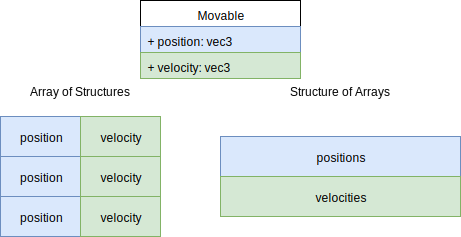
\includegraphics[width=\linewidth]{BAC-DOD1}}
	\caption{Příklad transformace pole struktur na strukturu polí.}
	\label{Fig:SOAASO}
\end{figure}

Základem \emph{DOD} je důkladná analýza aplikačních dat -- jejich obor hodnot, transformace, definice vstupních dat, požadovaný výstup atp. Často je využíváno datové struktury pole, jehož vlastnosti umožňují rychlou iteraci. Mezi výhody \emph{DOD} patří také dobrá lokalita dat a odkazů, což umožňuje efektivní využití procesorových \emph{cache}. Díky těmto vlastnostem se \emph{DOD} stále častěji používá v herním průmyslu\cite{DataOrientedDesignDice}\cite{DataOrientedDesignCppCon}.

Entitní systém navržený v této práci vychází z principů \emph{DOD} -- \emph{datově orientovaná kompozice}\cite{DODComponents}. Blíže se tímto způsobem skládání \emph{entit} zabývá sekce \ref{Chap:DOC}.

\section{Reprezentace entit}

Tato sekce obsahuje rozbor nejpoužívanějších způsobů reprezentace \emph{entit}\cite{EvolveHierarchy} a jejich \emph{chování}. Pod pojmem \emph{entita} je myšlen objekt ve virtuálním světě a \emph{chování} jsou operace, které \emph{entita} dokáže provést -- pohyb, vykreslení, kolize atp.

Jednotlivé reprezentace jsou srovnány na příkladu jednoduché 2D \emph{shoot'em up} hry. Metody jsou hodnoceny na základě složitosti implementace, návrhu s jejich použitím a výhodnosti z pohledu hardware. Závěry zde vyvozené jsou primárně zaměřené na \emph{třídní} objektově orientované jazyky (\emph{C++}, \emph{JAVA}, \emph{Python} atp.), ale částečně je lze aplikovat i na \emph{objektově orientované} programovací jazyky obecně.

\subsection{Objektově orientovaná hierarchie}

Pod pojmem \emph{objektově orientovaná hierarchie} (\emph{OOH} \cite{GameDesignPatterns}) je míněn způsob skládání nových typů entit za využití \emph{dědičnosti} a často také \emph{polymorfismu}. Příklad hierarchie, navržené pro ukázkovou 2D hru, lze vidět na obr. \ref{Fig:OOPHierarchy}. V kořenu stromu hierarchie je, v případě \emph{OOH}, bázová třída, která umožňuje uniformní skladování entit. Konkrétní entity, které existují v herním světě, jsou listy ve stromy dědičnosti.

Množina akcí entity je nastřádána průchodem stromu dědičnosti od kořene k listu, kde se konkrétní entita nachází. Existují dva často používané způsoby definice těchto akcí. První z nich je přímá definice metody v děděné třídě, tohoto je využíváno v případě akcí, které nezávisí na typu entity -- např. vykreslení. Druhým je potom využití polymorfizmu -- virtuálních metod.

\begin{figure}[H]
	\tmpframe{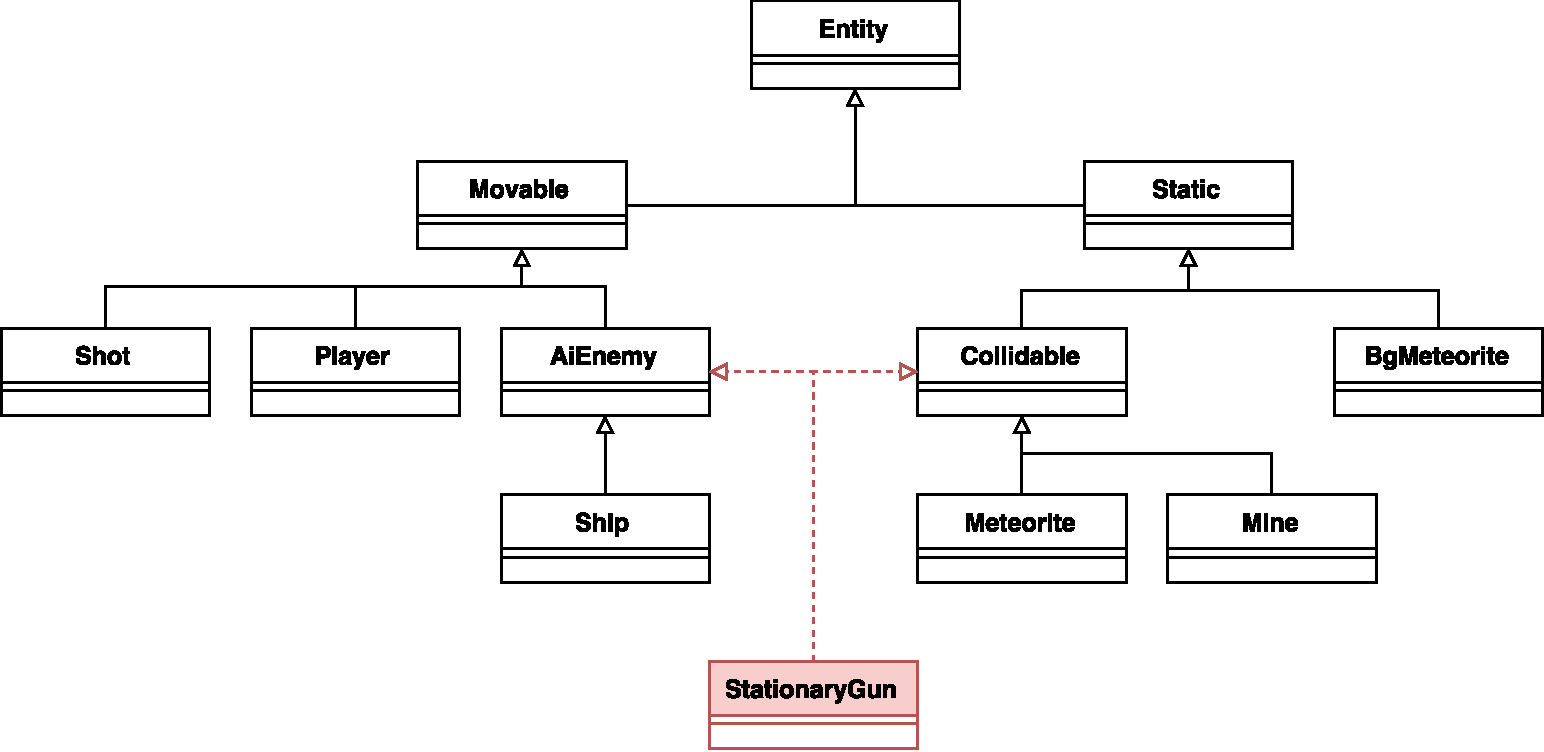
\includegraphics[width=\linewidth]{BAC-OOP1}}
	\caption{Příklad objektově orientované hierarchie.}
	\label{Fig:OOPHierarchy}
\end{figure}

Hierarchie dědičnosti, která je v tomto příkladě použita lze vidět na obr. \ref{Fig:OOPHierarchy} -- pouze ilustrační, pro předvedení problémů. Bázová třída \textbf{Entity} obsahuje kód pro vykreslování, dále se hierarchie dělí na entity pohyblivé a statické. Prvním problémem je umístění entit, které jsou v pozadí -- nelze do nich narazit. Dalším příkladem problémů s \emph{OOH} je přidání třídy \textbf{StationaryGun} (nepohyblivá zbraň), u které není optimální třída, ze které by měla dědit.

Pro příklad využití paměti je využit seznam pohybujících se entit, jejichž pozice musí být každý snímek hry aktualizována o jejich rychlost. Ilustrace možné organizace paměti lze vidět na obr. \ref{Fig:OOPMemory}. Hlavní seznam obsahuje ukazatele na entity, které je potřeba aktualizovat. Instance jednotlivých konkrétních typů jsou uloženy ve vlastních seznamech.

\begin{figure}
	\tmpframe{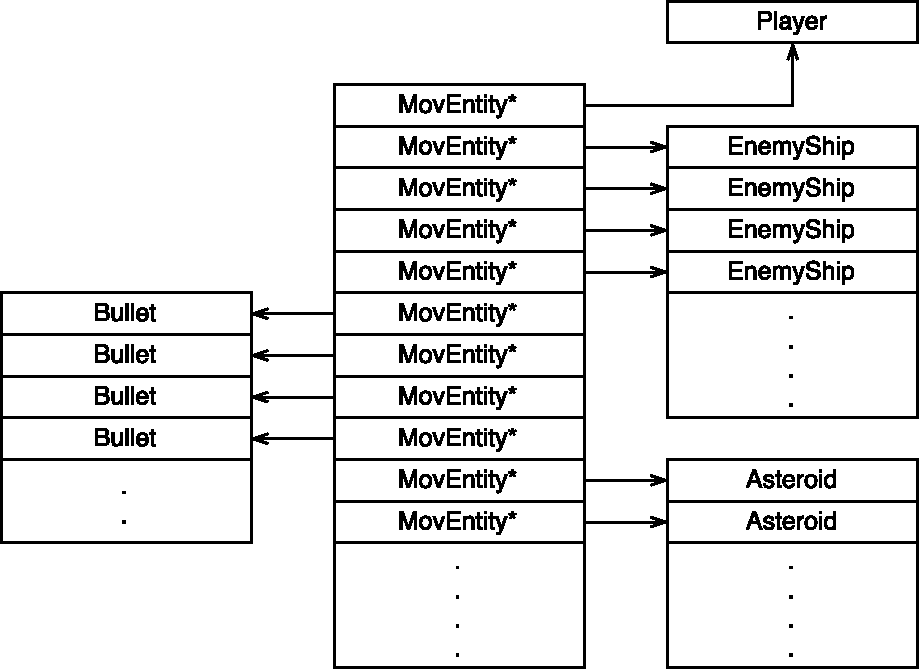
\includegraphics[width=\linewidth]{BAC-OOP2}}
	\caption{Obsah paměti u objektově orientovaných hierarchií.}
	\label{Fig:OOPMemory}
\end{figure}

Při operaci aktualizace je iterováno přes hlavní seznam ukazatelů a na každý objekt je zavolána metoda, která aktualizuje pozici o jeho rychlost. Postup práce s hlavní pamětí a \emph{cache} je následující \footnote{Postup neuvažuje různé vrstvy paměti \emph{cache} a předpokládá, že k požadovanému bloku paměti zatím nebylo přistoupeno. Velikost řádku vyrovnávací paměti je nastavena tak, aby nedošlo k překrytí paměti ukazatelů a paměti instancí.}. Prvním krokem je načtení bloku paměti o velikosti řádku vyrovnávací paměti (\emph{cache}), který obsahuje požadované ukazatele. Následuje dereference prvního z ukazatelů, která zapříčiní čtení dalšího řádků paměti, který již obsahuje iterované objekty. Ilustrace obsahu paměti \emph{cache} lze vidět na obr. \ref{Fig:OOPCache}. Díky způsobu, kterým jsou entity skládány, obsahují jednotlivé objekty kromě požadovaných informací -- pozice a rychlost -- také data, která nejsou používána. Výsledkem je neoptimální využití procesorových \emph{cache} \cite{DataOrientedDesignDice}.

\begin{figure}
	\tmpframe{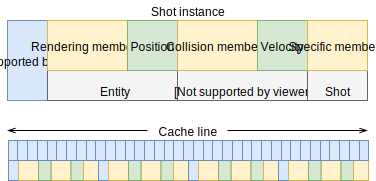
\includegraphics[width=\linewidth]{BAC-OOP3}}
	\caption{Využití procesorové \emph{cache} při použití objektově orientované entitní hierarchie.}
	\label{Fig:OOPCache}
\end{figure}

Komunikace jednotlivých částí je při použití \emph{OOH} implicitní -- pomocí \emph{public} a \emph{protected} členů. 

\pagebreak

\noindent Mezi výhody \emph{OOH} patří: 
\begin{itemize}
	\item Jednoduchá implementace.
	\item Podpora tříd zabudována do mnoha programovacích jazyků.
	\item Použití standardních návrhových metod z objektově orientovaného návrhu.
	\item Implicitní propojení a komunikace mezi děděnými částmi.
\end{itemize}

\noindent Její nevýhody jsou: 
\begin{itemize}
	\item Akumulace stavu a chování, které není nutně entitou vyžadováno.
	\item Duplikace kódu v různých větvích stromu dědičnosti.
	\item Zvyšující se složitost umisťování nových typů entit.
	\item Typy entit jsou specifikovány ve zdrojovém kódu.
	\item Statické typování \footnote{Může být výhodou v některých případech, např. optimalizace, které vykonává překladač.}, nemožnost tvorby nových typů za běhu programu.
\end{itemize}

\subsection{Objektově orientovaná kompozice}

Pod pojmem \emph{objektově orientovaná kompozice} (\emph{OOC} \cite{GameDesignPatterns}) je myšlena tvorba entit z menších částí -- komponent -- kde komponenty obsahují data i množinu proveditelných akcí. Entita je při použití \emph{OOC} kontejner, který obaluje seznam komponent (kompozice). Příklad návrhu množiny komponent lze vidět na obr. \ref{Fig:OOCHierarchy}, kontejnerovou třídou je v tomto případě \textbf{Entity}.

Množinu akcí, které lze nad entitou provést je definována komponenty, které jsou v entitě přítomny. Každá komponenta obsahuje, kromě dat, také akce, které lze nad entitou, která danou komponentu obsahuje, provést.

Tato metoda je často používaná (\emph{composition over inheritance}) v návrhu software a je mezikrokem od \emph{objektově orientované hierarchie} k \emph{datově orientované kompozici}. 

\begin{figure}
	\tmpframe{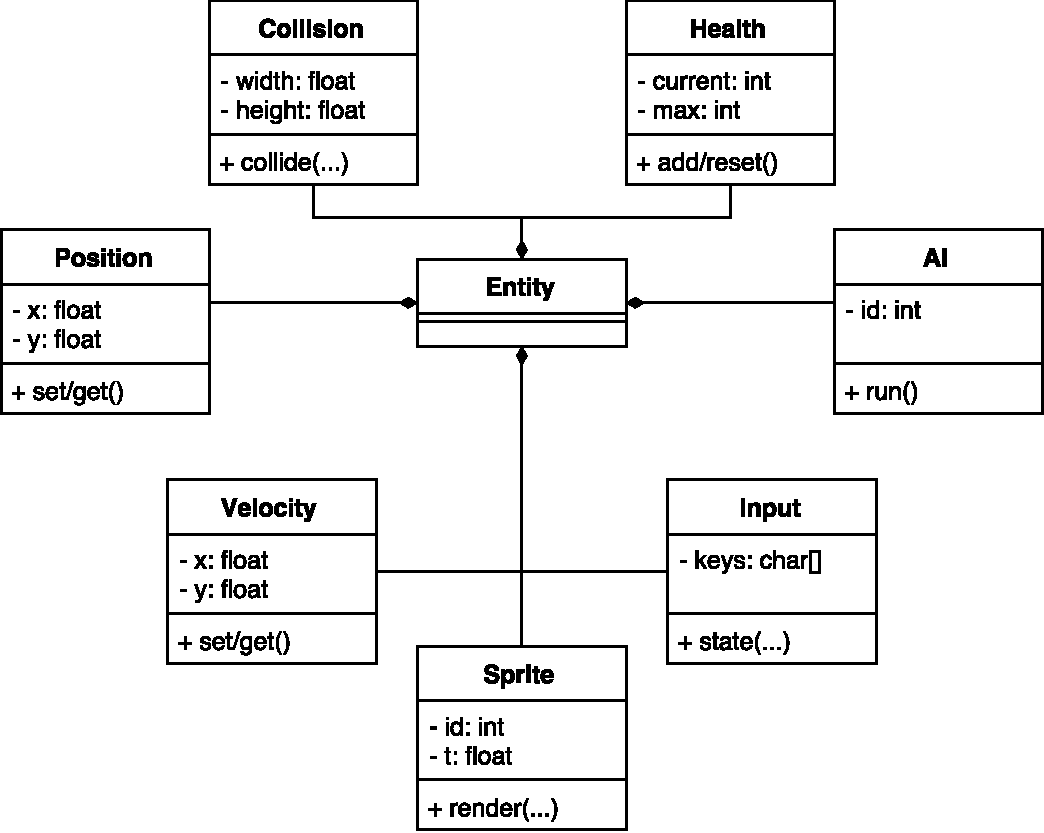
\includegraphics[width=\linewidth]{BAC-OOC1_1}}
	\caption{Příklad objektově orientované kompozice.}
	\label{Fig:OOCHierarchy}
\end{figure}

Příkladem využití těchto komponent, pro implementaci stejné množiny konkrétních entit, jako v případě použití \emph{OOH}, lze vidět na obr. \ref{Fig:OOCEntity}. Oproti využití dědičnosti se zde již lze jednoduše vyhnout problému s umístěním entit do stromu dědičnosti. Přidání typu \textbf{StationaryGun} je již také bezproblémové, díky možnosti libovolné kombinace jednotlivých komponent.

\begin{figure}
	\tmpframe{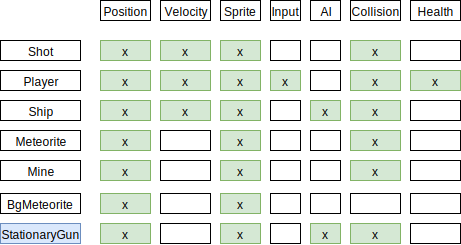
\includegraphics[width=\linewidth]{BAC-OOC1_2}}
	\caption{Využití kompozice pro tvorbu herních objektů. Konkrétní typy entit jsou zde reprezentovány řádky, jednotlivé komponenty jsou potom sloupce. Přítomnost komponenty je vyznačena znakem \uv{\emph{x}}.}
	\label{Fig:OOCEntity}
\end{figure}

Existuje mnoho způsobů, jak tuto základní myšlenku kompozice z menších částí implementovat. Jednou z možností je vyhradit pro každý typ komponenty pozici v seznamu ukazatelů \footnote{Mezi další způsoby patří mapy nebo dynamické seznamy. Možným řešením je také použití obecných ukazatelů a typových proměnných. }. V tomto návrhu je entita redukována na seznam ukazatelů, kde každá komponenta je buď přítomna (ukazatel je nastavený), nebo nepřítomna (ukazatel je \emph{NULL}). Výhodou této implementace je rychlost. Primární nevýhodou je potom neefektivní využití paměti, pro větší množství druhů komponent. Ilustraci této implementace lze vidět na obr. \ref{Fig:OOCImpl}. 

\begin{figure}
	\tmpframe{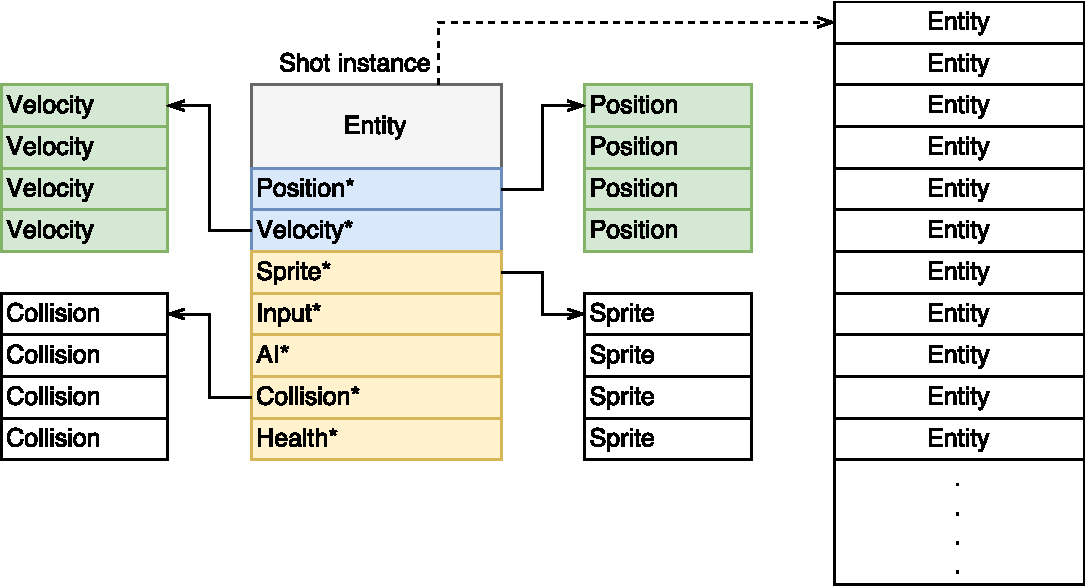
\includegraphics[width=\linewidth]{BAC-OOC2}}
	\caption{Obsah paměti u objektově orientované kompozice. Zde je entita implementována pomocí seznamu ukazatelů.}
	\label{Fig:OOCImpl}
\end{figure}

Jako příklad práce s pamětí je použita iterace nad seznamem entit, u kterých je nutno provést aktualizaci pozice, podle jejich rychlosti. V tomto příkladě je použita implementace pomocí statického seznamu ukazatelů, podle obr. \ref{Fig:OOCImpl}.

Podobně, jako u použití \emph{OOH}, je zde iterováno přes seznam, který však tentokrát obsahuje již jednotlivé instance typu \textbf{Entity} \footnote{Předpokládá se, že všechny entity obsahují komponenty typu \textbf{Position} a \textbf{Velocity}}. Využití vyrovnávací paměti, za stejných předpokladů, jako u příkladu v případě \emph{OOH}, je následující. Nejdříve je načten seznam entit a jejich ukazatelů na jednotlivé komponenty. Požadovaná operace potřebuje pouze ukazatele na komponenty typu \textbf{Position} a \textbf{Velocity}, ostatní jsou v tomto případě zbytečné \footnote{Záleží na implementaci, tuto neefektivitu je možné řešit optimalizacemi. }. Následuje přístup k požadovaným komponentám skrz ukazatele v první entitě. Tímto je načten blok paměti, pro každou komponentu, do vyrovnávací paměti. Po provedení operace nad první entitou a přístupu k dalším jsou již následující komponenty přístupné z \emph{cache}. 

\begin{figure}
	\tmpframe{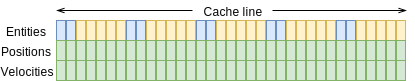
\includegraphics[width=\linewidth]{BAC-OOC3}}
	\caption{Využití procesorové \emph{cache} při použití objektově orientované kompozice.}
	\label{Fig:OOCCache}
\end{figure}

Komunikace mezi jednotlivými komponenty je při použití \emph{objektově orientované kompozice} problematické. Příkladem by mohla být \emph{umělá inteligence}, která potřebuje změnit rychlost entity. Jelikož jsou jednotlivé komponenty samostatné (\emph{encapsulation}) objekty, oddělené od ostatních komponent, které jsou součástí stejné entity, není mezi nimi možná přímá komunikace. Jedním možným řešením je přidání systému zpráv \footnote{Zprávy, ale i události jsou možným řešením.}, který má přístup k entitě, jako celku a předat odkaz na tento systém jednotlivým komponentám.

\noindent Mezi výhody \emph{OOC} patří: 
\begin{itemize}
	\item Uniformní instance všech typů entit, liší se pouze v přítomných komponentách.
	\item Lepší využití procesorových \emph{cache}.
	\item Možnost definování nových typů entit za běhu, použitím kompozice.
	\item Definice typů entit v datech.
	\item Komponenty, které entita vlastní, jsou přístupny z jednoho místa.
	\item Odstraněna duplikace kódu a akumulace nechtěného stavu.
\end{itemize}

\noindent Její nevýhody jsou: 
\begin{itemize}
	\item Složitější implementace, většinou bez podpory v programovacím jazyce.
	\item Komunikace mezi komponentami není implicitní, je nutno ji implementovat. 
\end{itemize}

\subsection{Datově orientovaná kompozice}
\label{Chap:DOC}

\emph{Datově orientovaná kompozice} (\emph{DOC}) je dalším krokem v rozdělování entit do logických celků -- do komponent. Podobně, jako \emph{objektově orientovaná kompozice}, \emph{DOC} rozděluje entity do menší části (komponenty), což umožňuje lepší modularitu výsledného software. Oproti \emph{OOC} však jednotlivé komponenty neobsahují žádnou logiku \footnote{Logikou je v tomto případě myšleno kód, který pracuje na vyšší úrovni, než pouze s daty dané komponenty. Blíže k tomuto v \ref{Chap:EntitySystem}}.

Množinu akcí, kterou lze nad entitou vykonat, je opět definována přítomnými komponentami. Jelikož komponenty samy o sobě neobsahují logiku, je nutno akce definovat v okolním kódu. Jedním způsobem je přímý přístup ke komponentám a jejich datům, tato metoda bude použita v následujícím příkladě. Pro rozsáhlejší aplikace, kde je třeba lepší kontrola nad přístupy k jednotlivým komponentám, lze například využít \emph{systémy}, které implementují akce nad komponenty \footnote{Tato metoda je blíže popsána v sekci \ref{Chap:EntitySystem}}. Tento způsob je využit i v návrhu \emph{entitního systému}, o kterém je napsána tato práce.

\begin{figure}
	\tmpframe{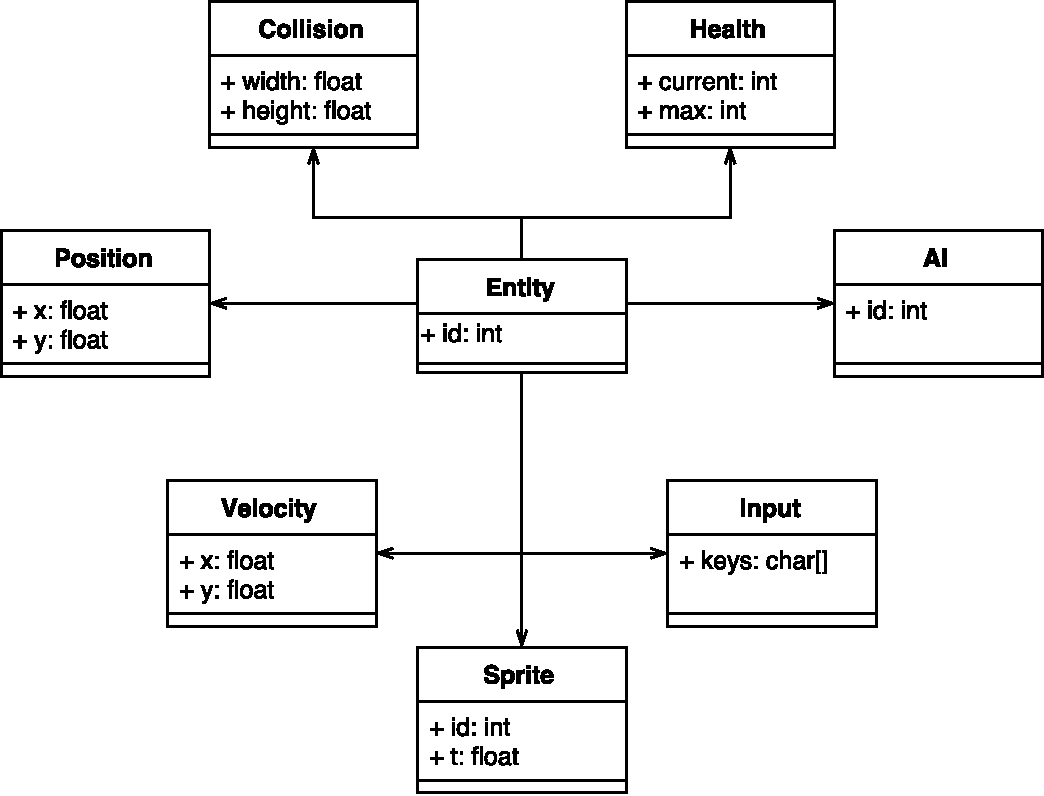
\includegraphics[width=\linewidth]{BAC-DOC1_1}}
	\caption{Příklad datově orientované kompozice.}
	\label{Fig:DOCHierarchy}
\end{figure}

Příklad návrhu entity a komponent lze vidět na obr. \ref{Fig:DOCHierarchy}. Mezi důležité změny, oproti \emph{OOC}, patří veřejný (\emph{public}) přístup ke členům entit. Entita je v tomto návrhu \footnote{Toto je pouze jeden způsob implementace \emph{datově orientované kompozice}.} reprezentována číslem (identifikátor), pomocí kterého lze komponenty jednoznačně přiřadit k entitám, které je vlastní. Implementace konkrétních entit je konceptuálně stejná, jako při použití \emph{objektově orientované kompozice}, příklad lze vidět na obr. \ref{Fig:OOCEntity}.

\begin{figure}
	\tmpframe{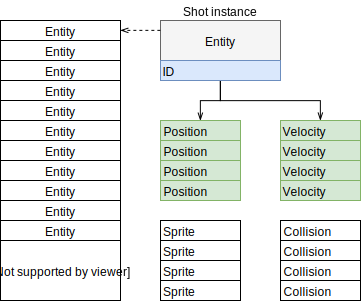
\includegraphics[width=\linewidth]{BAC-DOC2}}
	\caption{Obsah paměti u datově orientované kompozice.}
	\label{Fig:DOCMemory}
\end{figure}

Příklad organizace paměti, při použití \emph{DOC}, lze vidět na obr. \ref{Fig:DOCMemory}. Entity jsou uchovávány v homogenním seznamu. Jednotlivé identifikátory entit je možné mapovat na komponenty přímou indexací polí komponent.

\begin{figure}
	\tmpframe{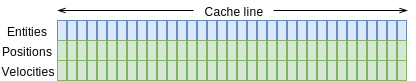
\includegraphics[width=\linewidth]{BAC-DOC3}}
	\caption{Využití procesorové \emph{cache} při použití datově orientované kompozice.}
	\label{Fig:DOCCache}
\end{figure}

Pro ukázku práce s vyrovnávací paměti je opět použit příklad iterace nad seznamem entit, které je nutno posunout v prostoru, podle jejich rychlosti. Pro vykonání této akce je tedy nutný přístup ke komponentám typu \textbf{Position} a \textbf{Velocity}. Nejdříve je opět přistoupeno k poli entit, čímž je načten příslušný řádek do vyrovnávací paměti. Jelikož je mapování identifikátorů entit realizováno pomocí přímé indexace \footnote{Za předpokladu, že identifikátory všech iterovaných entit nedovolují díry v poli komponent.} je možné po načtení řádku \emph{cache} pro dané dva typy komponent již následující přístupy do paměti realizovat přímo z vyrovnávací paměti. Obrázek \ref{Fig:DOCCache} obsahuje ilustraci stavu procesorové \emph{cache}.

Komunikace mezi jednotlivými částmi je v případě \emph{datově orientované kompozice} rozdělená do dvou úrovní. První z nich, komunikace mezi komponentami, je vyřešena implicitně, jelikož akce mohou přistupovat k několika komponentám. Druhou je potom komunikace mezi zprostředkovateli akcí (např. \emph{systémy}). Tento typ komunikace je možné opět řešit pomocí systému zpráv, nebo událostí. 

\noindent Mezi výhody \emph{DOC} patří: 
\begin{itemize}
	\item Efektivní skladování entit, které jsou reprezentovány identifikátorem.
	\item Lepší využití procesorových \emph{cache}.
	\item Možnost definování nových typů entit za běhu, použitím kompozice.
	\item Definice typů entit v datech.
	\item Odstraněna duplikace kódu a akumulace nechtěného stavu.
	\item Možnost efektivní implementace akcí, mimo komponenty.
	\item Možná vysoká úroveň optimalizace celého systému.
\end{itemize}

\noindent Její nevýhody jsou: 
\begin{itemize}
	\item Bez podpory v programovacích jazycích \footnote{Vzniká programovací jazyk, který bude tento typ kompozice podporovat \cite{OOHLang}.}.
	\item Náročná implementace.
\end{itemize}

\pagebreak

\noindent Mezi další vlastnosti patří:
\begin{itemize}
	\item Ztráta abstrakce při práci s komponentami.
	\item Možnosti \emph{serializace} entit a komponent.
	\item Akce mohou přistupovat k několika komponentám.
\end{itemize}

\section{Entity-Component-System}
\label{Chap:EntitySystem} 

Entitní systémy, postavené za použití \emph{datově orientované kompozice}, s využitím \emph{systémů} pro generování chování, se nazývají \emph{Entity-Component-System}  \footnote{Často používaným označením je také \uv{component base entity system},  \uv{Component-Entity-System}, nebo i \uv{Entity System}.}. Tato část obsahuje popis obecných konceptů tohoto typu systémů, a vlastností, které z nich vyplývají.

\subsection{Motivace a koncepty}

\emph{Entity-Component-System} (\emph{ECS} \cite{WhatIsECS} \cite{UnderstandingECS}) je programovací paradigma \cite{EntitySystemsFuture}, založené na kompozici \footnote{Oproti \uv{Object Oriented Programming}, které využívá dědičnosti.}.  Základní myšlenkou je separace logiky (\emph{systémy}) a dat (\emph{entity}, \emph{komponenty}), čímž je umožněna jemnější modularita, celý entitní systém lze přirovnat k \emph{relační databázi}. Tato metoda vychází z \emph{datově orientované kompozice}, která je podrobněji popsána v části \ref{Chap:DOC}. 

Entita je základním stavebním blokem \cite{EntitySystemsFuture}, který lze přirovnat k objektu z \emph{objektově orientovaného} návrhu. Oproti objektům nejsou však entity tvořeny z předem daného vzoru (např. třídy). Jejich chování a data, definují komponenty, které jsou k dané entitě přiřazeny. Entity lze reprezentovat pomocí jednoznačných identifikátorů (čísel), které mají podobnou funkci, jako \emph{primární klíče} v databázi, ilustrace tohoto přirovnání lze vidět na obr. \ref{Fig:ECSDB}.

Komponenty jsou základními nosiči dat \footnote{Některé typy komponent -- např. značky -- nemusí nutně ani data obsahovat.} v \emph{ECS}. Po přiřazení komponent k entitám však mají komponenty i důležitější funkci -- určují chování entit. Kromě explicitních dat obsažených v komponentách existuje také, implicitně, informace o tom, zda určitá entita obsahuje (má přiřazen) daný typ komponenty. Často používaným názvem pro komponenty, je také \uv{aspekt} \cite{EntitySystemsFuture}. Každá entita má k sobě přiřazeno $0-1$ komponent daného typu, kde přítomnost komponenty znamená, že entita splňuje daný aspekt. V přirovnání \emph{ECS} k \emph{relační databázi}, lze o komponentách smýšlet jako o sloupcích (obr. \ref{Fig:ECSDB}) tabulky entit.

\begin{figure}
	\tmpframe{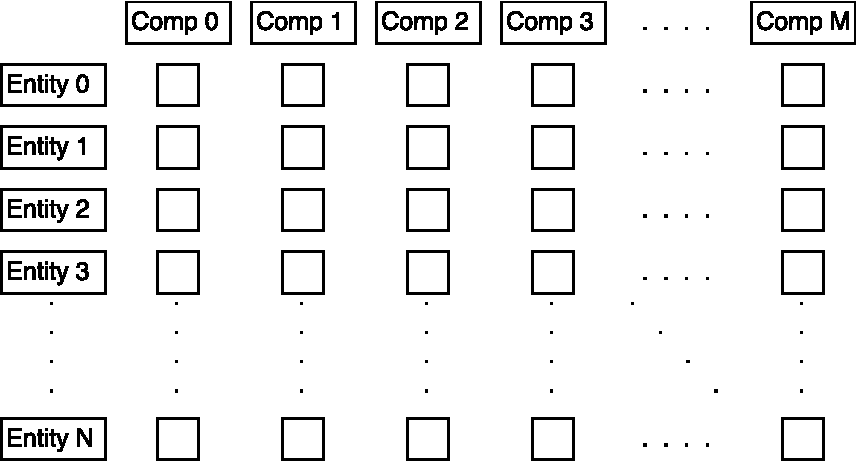
\includegraphics[width=\linewidth]{BAC-ECS1}}
	\caption{Entita reprezentována jako řádek v databázi. Primárním klíčem je identifikátor entity.}
	\label{Fig:ECSDB}
\end{figure}

Pokud bychom pokračovali s přirovnáním k \emph{OOP} -- entity jsou jednotlivé objekty, komponenty umožňují polymorfizmus -- potom systémy implementují chování, nebo metody jednotlivých komponent. Pro mnoho různých typů dat, kde každý typ vyžaduje vlastní chování, je \emph{OOP} výhodné, protože je možné data i operace uložit do jednoho nerozdělitelného celku. Pokud je však nutné vykonat stejnou akci na velkém množství různých typů, \emph{OOP} není optimálním řešením a \emph{ECS} je v tomto případě vhodnější \cite{EntitySystemsFuture}. 

Každý systém provádí danou operaci na všech entitách, které obsahují požadované komponenty (\emph{aspekty}). Základní schéma systému lze vidět na obr. \ref{Fig:ECSSystem}. Výběr vhodných entity je proveden pomocí filtru, který operuje nad přítomností jednotlivých komponent (obr. \ref{Fig:ECSFilter}).

\begin{figure}[H]
	\tmpframe{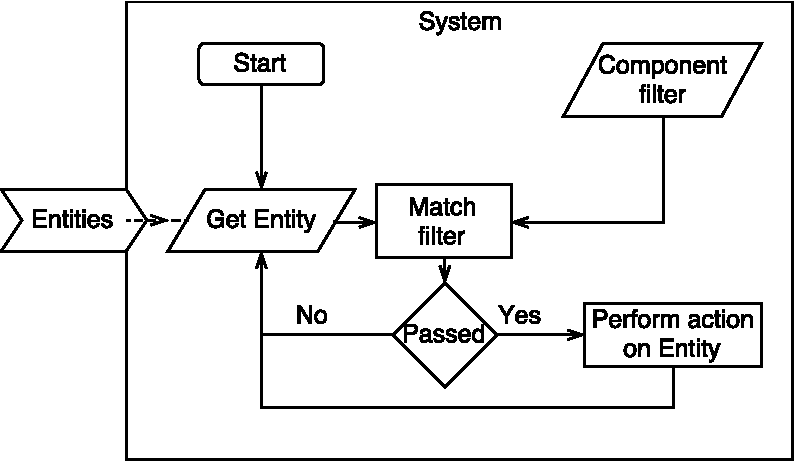
\includegraphics[width=\linewidth]{BAC-ECS2}}
	\caption{Vstupem \emph{systému} jsou entity, ze kterých si vybere pouze ty, které mají odpovídající komponenty. Na vybraných entitách provádí požadované akce.}
	\label{Fig:ECSSystem}
\end{figure}
\begin{figure}[H]
	\tmpframe{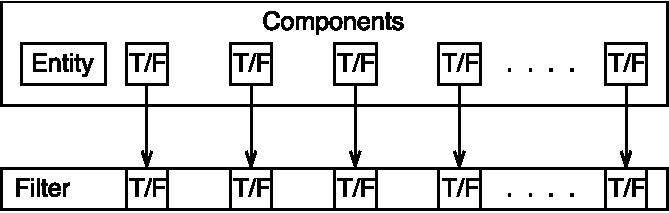
\includegraphics[width=\linewidth]{BAC-ECS3}}
	\caption{Filtr operuje nad entitou a informací o přítomnosti komponent.}
	\label{Fig:ECSFilter}
\end{figure}

\subsection{Vlastnosti}

Důvody, proč se \emph{ECS} často používá při návrhu moderních her je mnoho a většina z nich vzniká díky striktnímu oddělení logiky a dat. Komponenty je možné skladovat v sekvenčních blocích paměti, toto zlepšuje efektivitu využití procesorových \emph{cache}. Lokalita dat se vztahuje i na instrukce \cite{InstrAreData} \footnote{\emph{Instrukční cache} \cite{CpuMemoryGap}} a díky opakovanému provádění stejných operací nad velkým počtem entit dochází k vyšší efektivitě využití \emph{instrukční cache}. 

Inherentní modularita \emph{ECS} dovoluje lepší dělení práce ve velkých týmech vývojářů. Každý systém musí předem specifikovat, o jaké entity (které aspekty musí splňovat) má zájem, tímto je zamezeno nechtěnému ovlivňování okolního kódu. Další výhodou, z pohledu organizace kódu, je přímočará \emph{refaktorizace} systémů a komponent.

Jelikož komponenty obsahují pouze čistá data, bez propojení do externích modulů, je možné přistupovat k entitnímu systému také z vestavěného skriptovacího jazyka (např. \emph{LUA}). Skriptovací jazyky bývají hojně využívány jako součást \uv{gameplay} \footnote{Kód, který se stará o interakce virtuálních objektů ve hře.} funkcí, nebo \emph{umělé inteligence}. Pokročilou vlastností \emph{ECS} může také být přidávání nových typů komponent za běhu aplikace. Tyto, ale i další (např. \emph{serializace} komponent), funkce umožňují rychlé prototypování nových herních mechanik.

Při správném rozvržení systémů a jejich požadovaných aspektů, je možné zaručit, že k ostatním komponentám nebude přistupováno. Toto umožňuje dosáhnout vyšší úrovně paralelizace celého systému, i přestože několik systémů může v jeden čas přistupovat ke stejné entitě. Paralelizace je dále podporována opakovaným prováděním stejných akcí nad velkým množstvím entit, které lze rozdělit na různá vlákna a zpracovat je odděleně.

\section{Paralelizmus}
\label{Chap:Parallelism}

Vývoj moderních procesorů se ubírá směrem zvyšování počtu výpočetních jader \cite{CPUPerfHistory} a proto i moderní aplikace musí být schopné tato jádra využít. To je zvláště pravda pro vývoj her, které se snaží s hardware vytěžit maximální výkon. Paralelizace aplikací, jejichž části jsou úzce provázané je obzvláště problematické a proto vznikají nové způsoby tento typ software navrhovat -- jedním z nich je právě \emph{ECS}. 

Paralelizmus lze obecně rozdělit na 2 typy -- datový a úkolový \cite{KindsOfParallelism}. Při použití datového paralelizmu je prováděna jedna akce, na různých datech (obdoba \emph{SIMD} u procesorů). Opačným přístupem je paralelizmus úkolový \cite{TaskBasedParallelism}, u kterého mohou běžet různé operace nad stejnými daty (\emph{MISD}). Ve většině případů je však používáno kombinací těchto dvou přístupů. Speciálním případem je vyhrazení celého vlákna jednomu modulu -- např. manažer zvuku -- který vyžaduje nízké odezvy \cite{FrontierThreads}.

Výhodou paralelizmu je možnost rozložení práce na několik výpočetních jednotek, což umožňuje požadovanou akci provést rychleji. Využití paralelizmu však představuje mnoho nových typů problémů, které se u sekvenčního programování nevyskytují. Kromě obecně známých překážek, jako jsou synchronizace vláken, potenciální uváznutí (\emph{deadlock}), různých typů souběhu (\emph{race condition}), existují také problémy na hardwarové úrovni. Hlavním z nich je udržování koherence procesorových \emph{cache} \cite{CacheCoherence} a skrz to problém, který se nazývá \uv{false sharing} \cite{FalseSharing}. V případě, že několik vláken pracuje se stejným blokem paměti -- je načtený v jeho lokální vyrovnávací paměti -- je nutné \emph{cache} jednotlivých jader synchronizovat tak, aby každé z nich nepracovalo s jinými daty. Tento proces se nazývá \uv{udržování koherence vyrovnávacích pamětí}. Problém, který v tomto systému může nastat -- \uv{false sharing} -- vzniká v případě, kdy obě vlákna pracují nad stejnou pamětí \footnote{Paměť je součástí stejného řádku vyrovnávací paměti.}, ale nepracují se stejnými daty. Při každé změně bude nutno provést synchronizaci, i když není nutná, ilustraci tohoto jevu lze vidět na obr. \ref{Fig:PARFalseSharing}.

\begin{figure}
	\tmpframe{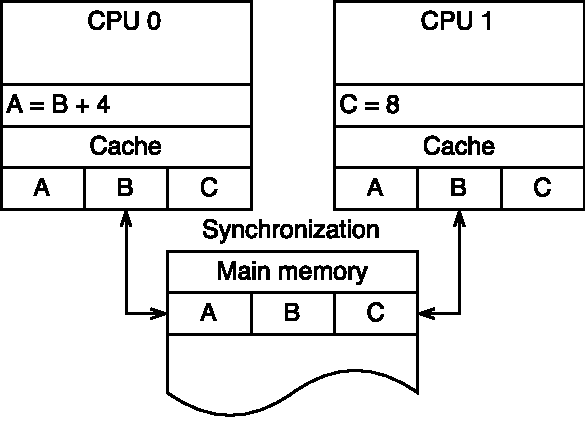
\includegraphics[width=\linewidth]{BAC-PAR0}}
	\caption{Udržování koherence vyrovnávací paměti a \uv{false sharing} \cite{FalseSharing}. Synchronizace \emph{cache} je prováděna mezi jednotlivými jádry, přes specializovanou sběrnici.}
	\label{Fig:PARFalseSharing}
\end{figure}

\emph{Entity-Component-System} paradigma je výhodné z pohledu více-jádrových systémů, díky možnosti téměř \cite{AmdahlLaw} dokonalé paralelizace na několika úrovních \cite{ParallelGame}. První úrovní paralelizace, kterou \emph{ECS} umožňuje, je datový paralelizmus, kde se uvnitř systému množina všech entit, které odpovídají požadavkům, rozdělí do množiny vláken, které mohou dané akce provádět odděleně \footnote{Některé typy akcí tento paralelizmus neumožňují - např. výpočet pozic objektů v grafu scény.}. Ilustrace principu, jak tento způsob pracuje lze vidět na obr. \ref{Fig:PARData}. Dalším způsobem paralelizace je možnost spouštět jednotlivé systémy na oddělených vláknech (obr. \ref{Fig:PARSystem}), tato metoda je ovšem použitelná pouze pro systémy, které nezapisují do komponent, které jsou zároveň používány v jiném systému. 

\begin{figure}
	\tmpframe{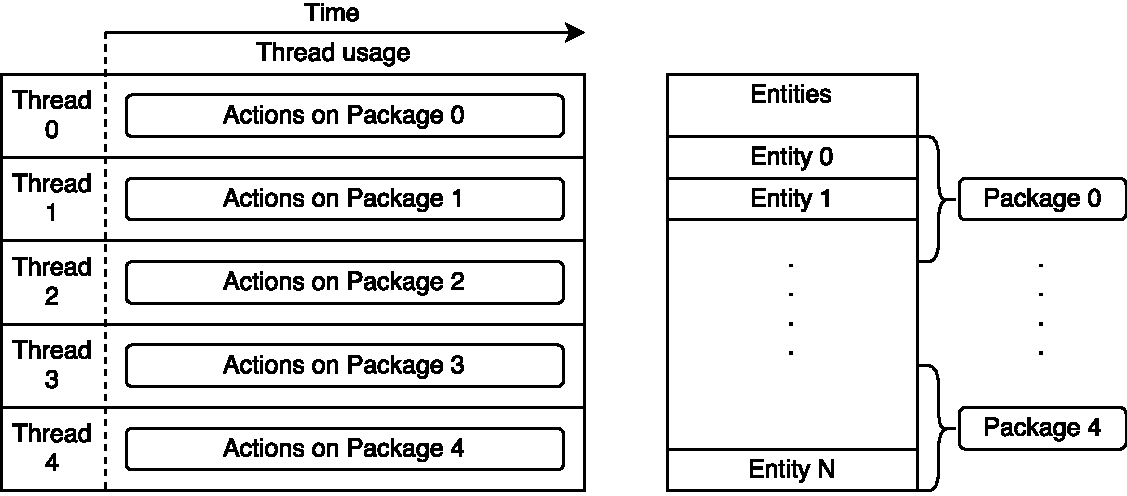
\includegraphics[width=\linewidth]{BAC-PAR1}}
	\caption{Paralelizmus uvnitř systémů je příkladem datového paralelizmu \cite{KindsOfParallelism}.}
	\label{Fig:PARData}
\end{figure}

\begin{figure}
	\tmpframe{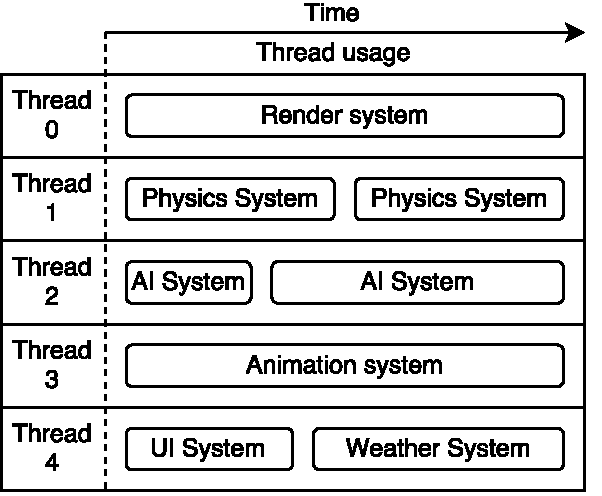
\includegraphics[width=\linewidth]{BAC-PAR2}}
	\caption{Paralelizmus na úrovni systémů, kdy několik systémů běží zároveň.}
	\label{Fig:PARSystem}
\end{figure}

Jednoduchý systém může pracovat způsobem transformační funkce, jejíž vstupní parametry jsou komponenty, které systém požaduje a výstupem je zápis (změna) jedné z těchto komponent. Jelikož je ovšem vhodné, při paralelním přístupu k aktuálnímu stavu herního světa, aby všechny systémy dokázaly přečíst původní data beze změn, lze funkci systémů změnit. Systémy mohou místo zápisu nových hodnot do stejných komponent (vstupů) zapsat výsledek do \uv{následujícího stavu} \cite{FrontierThreads} \footnote{Tento způsob je často používán ve funkcionálních jazycích.}. Při generování nového stavu je nutné určit okamžik, kde se následující stav stane stavem aktuálním, čímž se celý herní svět \uv{posune}.

\chapter{Návrh entitního systému}

Obsahem této kapitoly je popis návrhu entitního systému založeného na \emph{ECS} paradigmatu, které bylo představeno v předchozí kapitole. Nejdříve je prezentováno základní rozdělení systému na jednotlivé části a komunikace mezi nimi. Následuje popis návrhu podsystémů -- \emph{komponenty}, \emph{systémy} a \emph{entity}. Každá část obsahuje představení návrhu a jeho zdůvodnění. Následuje návrh paralelního přístupu k entitnímu systému a jeho tok řízení.

\section{Přehled a komunikace}

Entitní systém je, podobně jako \emph{ECS} paradigma, rozdělený do několika částí -- modulů -- kde cílem jednotlivých částí je zpráva některé z domén \emph{ECS}. Diagram reprezentující toto rozdělení lze vidět na obr. \ref{Fig:DESModules}. Mezi tyto moduly patří -- zpráva systémů a skupin, zpráva komponent, zpráva entit a zpráva akcí. Bližší popis a návrh jednotlivých částí obsahují následující části této kapitoly.

\begin{figure}[H]
	\tmpframe{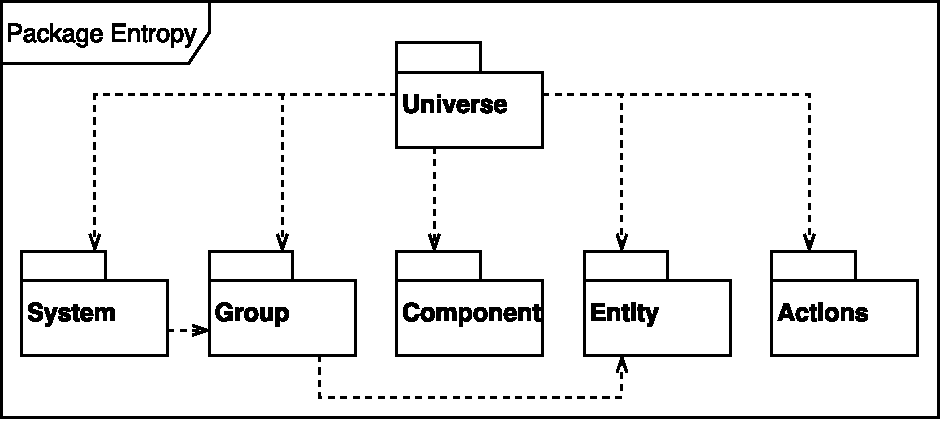
\includegraphics[width=\linewidth]{BAC-DES1}}
	\caption{Rozdělení entitního systému do modulů.}
	\label{Fig:DESModules}
\end{figure}

Funkcionalita celého systému je zastřešena třídou \textbf{Universe} (obr. \ref{Fig:DESUniverse}), skrz kterou je uživateli umožněn přístup k jednotlivým podsystémům. Pro každou operaci nad entitním systémem existuje metoda uvnitř třídy \textbf{Universe} -- tento návrh umožňuje jednotný vstupní bod. Nevýhodou je vysoké množství metod v této třídě. Další důležitou funkcionalitou třídy \textbf{Universe} je zprostředkování komunikace mezi jednotlivými moduly -- např. přidání komponenty má dvě části, skutečná operace nad nosičem komponent a úpravu metadat (obr. \ref{Fig:DESAddComp} a obr. \ref{Fig:DESAddEnt}). 

\begin{figure}[H]
	\tmpframe{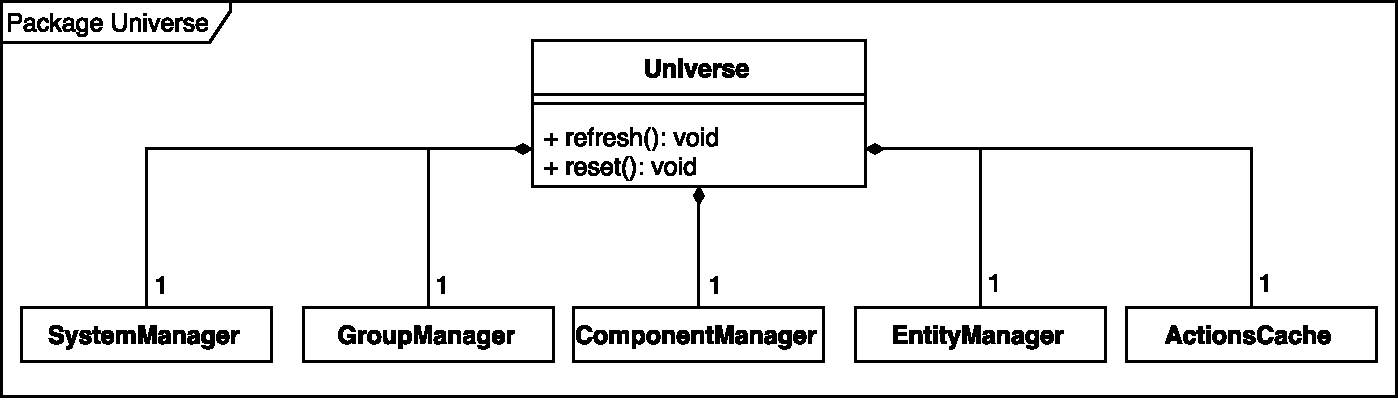
\includegraphics[width=\linewidth]{BAC-DES2}}
	\caption{Třída \textbf{Universe} je rozhraním entitního systému. Diagram neobsahuje specifikaci všech metod třídy, kvůli jejich vysokému počtu.}
	\label{Fig:DESUniverse}
\end{figure}

\section{Komponenty a jejich nosiče}

Komponenty jsou definovány jako základní datové jednotky v \emph{ECS}, kde každá entita má k sobě přiřazeno 0-1 komponent daného typu. Komponenty, jak s nimi pracuje tento návrh, mohou být jakékoliv třídy \footnote{Obecný typ komponenty je \textbf{Component}. Pokud to implementační jazyk vyžaduje, je možné požít abstraktní třídu stejného jména, ze které budou všechny konkrétní komponenty dědit.} a nemusí obsahovat žádné specifické akce. Každá komponenta má přiřazen unikátní identifikátor -- \textbf{CompId} -- tento identifikátor je neměnný po dobu běhu entitního systému. Komponenty by měly být pasivní datové struktury \footnote{\emph{Plain old data structure} (\emph{POD}) -- struktura reprezentovaná kolekcí hodnot.}, se kterými lze pracovat jako s čistou pamětí (přesuny, kopírování, atp.).

O zprávu komponent se stará podsystém zprávy komponent, jehož diagram lze vidět na obr. \ref{Fig:DESCompDiag}. Modul se skládá dvou částí -- registrace typů komponent a nosiče komponent. Veškerá komunikace probíhá skrz třídu \textbf{Component Manager}, která obsahuje metody pro registrace komponent a jejich následná asociace k entitám. 

V první fázi práce s tímto modulem je třeba registrovat typy komponent, které budou následně používány. Nové komponenty jsou registrovány pomocí metody \textbf{registerComponent} \footnote{Této metodě je třeba předat typ komponenty, která má být registrována, čehož lze docílit pomocí např. \emph{template} (C++), nebo \emph{generics} (Java)}, která vytvoří mapování z daného typu na jeho registr (\textbf{ComponentRegister}). Tohoto registru je následně využito pro získání specifického nosiče komponent.

\begin{figure}[H]
	\tmpframe{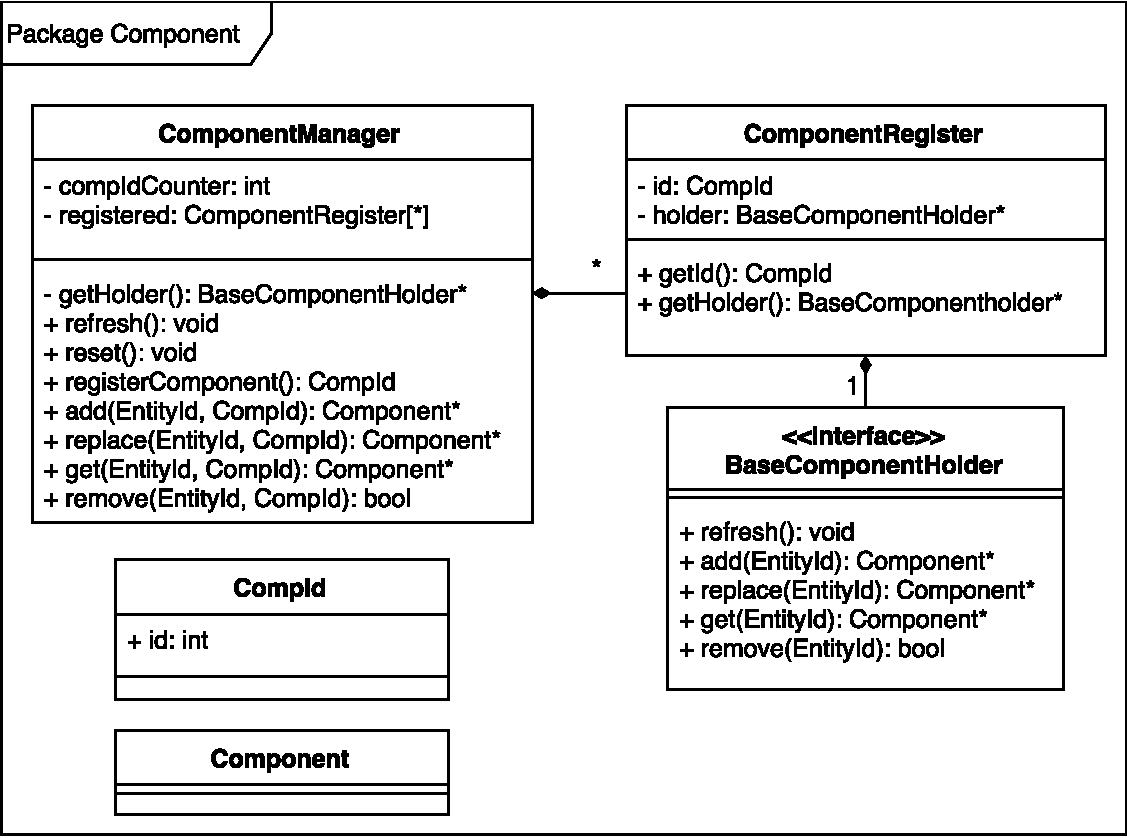
\includegraphics[width=\linewidth]{BAC-DES5}}
	\caption{Diagram tříd podsystému zprávy \emph{komponent}.}
	\label{Fig:DESCompDiag}
\end{figure}

Každý typ komponent je uložen ve vlastním kontejneru -- tzv. nosič komponent. Nosičem je třída, která dědí z \textbf{BaseComponentHolder} a implementuje všechny požadované operace, přičemž si může každá komponenta zvolit typ nosiče \footnote{Opět pomocí mechanizmu \emph{template}, nebo obdobných vlastností jiných jazyků.}. Hlavní funkcí nosiče je mapování identifikátorů entit (\textbf{EntityId}) na přiřazené komponenty. 

Různé implementace nosičů, specifické pro určené komponenty, umožňují vyšší úroveň optimalizace pro předpokládané využití komponent. Pokud je např. jisté, že téměř všechny entity budou obsahovat určitý typ komponenty, je možné implementovat nosič jako jednoduché pole, kde mapovací funkcí je prostá indexace komponent pomocí identifikátoru entit. Naopak, pokud je předpokladem, že komponenta bude využívána nízkým počtem entit, nosič může být implementován jako strom, kde klíčem je identifikátor entity. Speciálním typem komponenty je \emph{značka} (\emph{tag}), která neobsahuje žádná data, ale vzniká implicitní informace o tom, zda má entita danou značku přiřazenu, čehož lze využít pro např. rozdělení entit do skupin.

\begin{figure}[H]
	\tmpframe{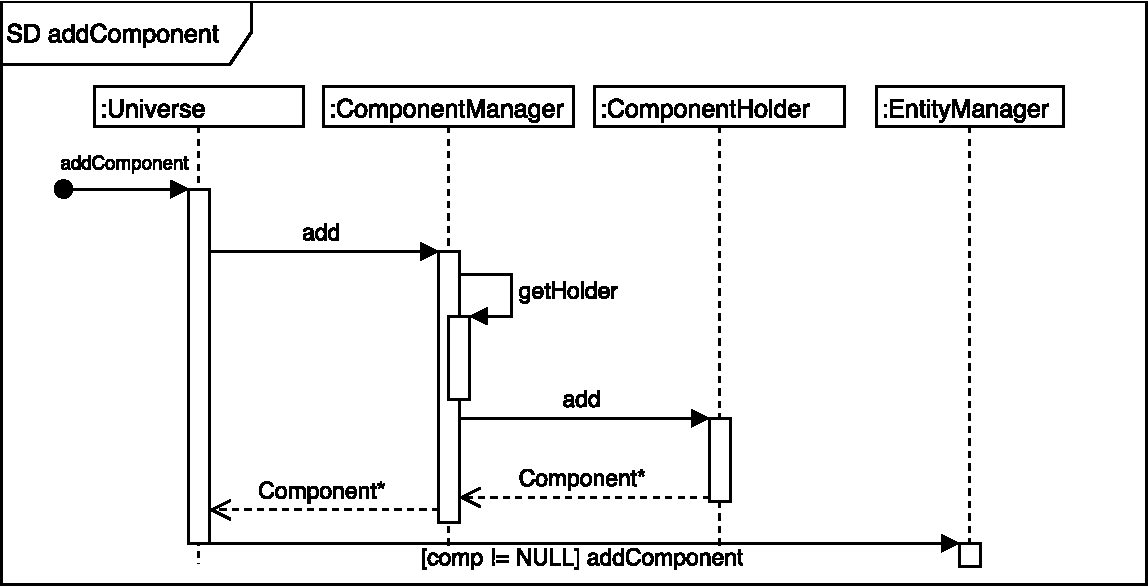
\includegraphics[width=\linewidth]{BAC-DES8}}
	\caption{Sekvenční diagram přidání komponenty, pokračuje na obr. \ref{Fig:DESAddEnt}.}
	\label{Fig:DESAddComp}
\end{figure}

Operace přidání komponenty je rozdělena do dvou částí, první z nich, která pracuje nad \textbf{ComponentManager} lze vidět na obr. \ref{Fig:DESAddComp}. Po úspěšném přidání komponenty následuje modifikace metadat, kterými se zabývá následující část kapitoly o návrhu.

\section{Reprezentace entit}

Entita, jako koncept z \emph{ECS}, je distribuovaný objekt, složený z komponent. Pro každou entitu existuje 1-0..1 mapování na každý typ komponent. Vyvstává tedy požadavek ne jednoznačný identifikátor entit, který by plnil funkci \emph{primárního klíče} v tabulce (obr. \ref{Fig:ECSDB}) entit.

Pro účely tohoto entitního systému je identifikátor složen ze dvou čísel -- ID a generace. ID je v tomto případě skutečný \emph{primární klíč}, pomocí kterého jsou jednotlivé řádky v tabulce entit indexované \footnote{Používá se tedy i při mapování komponent na entity uvnitř nosičů komponent.}. Generační číslo odlišuje různé generace entit, které zabíraly stejný řádek v tabulce (stejné ID) a je inkrementováno při každém smazání entity. Generační čísla identifikátorů, skrz které je přistupováno k systému jsou porovnány s aktuální generací dané entity, čímž je zamezen přístup ke smazaným entitám.

\begin{figure}[H]
	\tmpframe{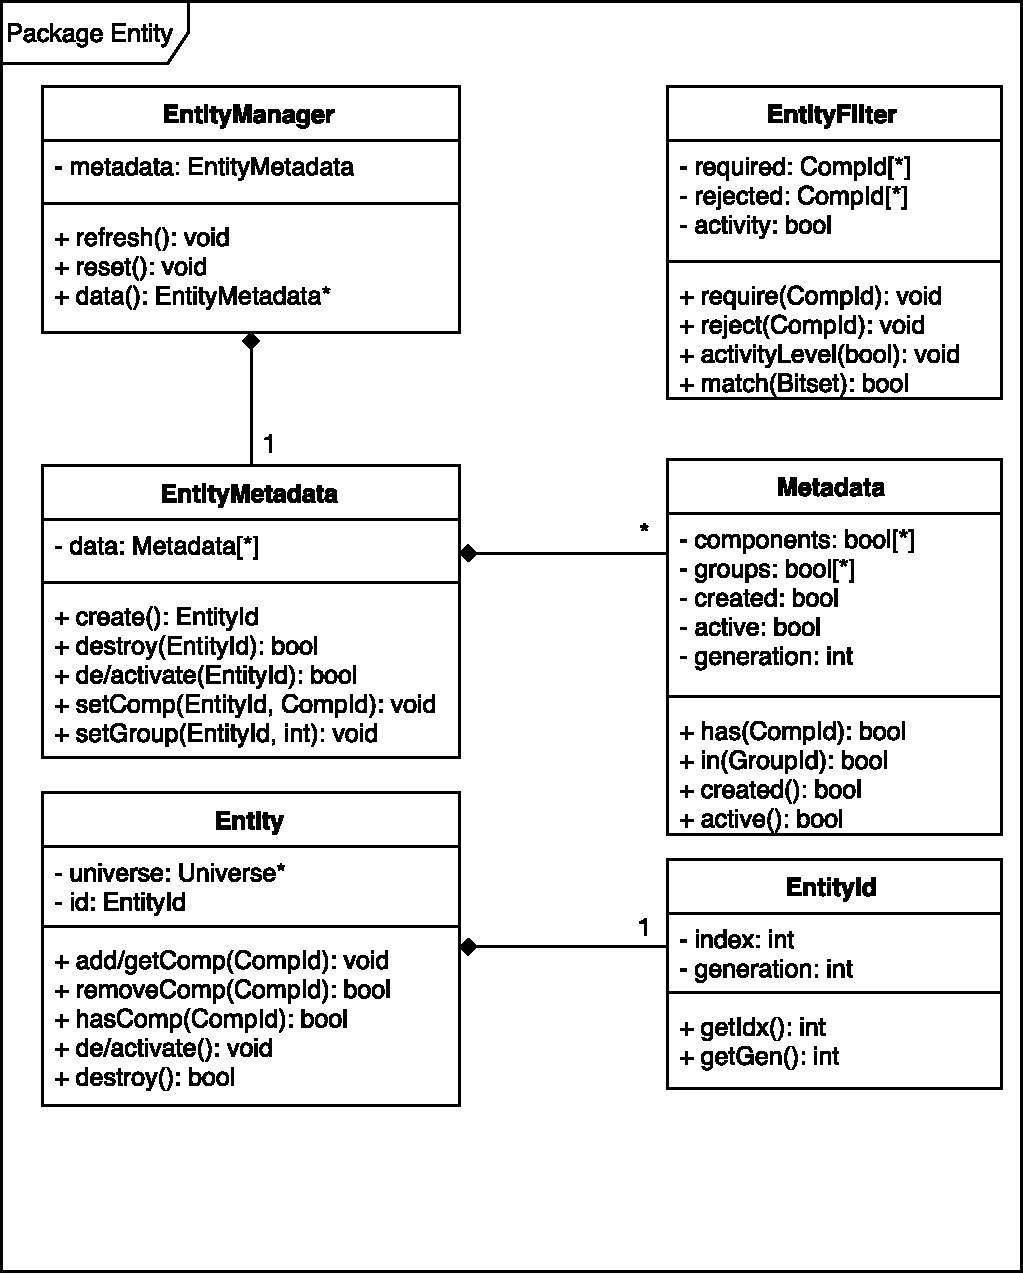
\includegraphics[width=\linewidth]{BAC-DES6}}
	\caption{Diagram tříd podsystému zprávy \emph{entit}.}
	\label{Fig:DESEntityDiagram}
\end{figure}

Podsystém zprávy entit, jehož diagram tříd lze vidět na obr. \ref{Fig:DESEntityDiagram}, lze přirovnat k relační databázi. Systém obsahuje jednu tabulku entit, kde každý řádek reprezentuje slot pro entitu. Identifikátor entity je složen z indexu řádku v tabulce a jeho generační hodnoty. Každý řádek obsahuje aktuální číslo generace a množinu \emph{bool} hodnot -- metadat. Ilustraci možné konfigurace tabulky metadat lze vidět na obr. \ref{Fig:DESMetadata}. Výhodou této reprezentace je konstantní složitost přístupu k metadatům dané entity \footnote{Indexace tabulky pomocí \emph{ID} části identifikátoru.}. 

Jelikož je mapováni identifikátorů entit na komponenty již součástí nosičů komponent, tabulka již tuto informaci nemusí obsahovat. Výhodné je však udržování informace o existenci komponent pro jednotlivé entity, které může být použito pro efektivní filtrování entit. Udržování tohoto typu informace je možné díky jednotnému rozhraní pro práci s komponenty (\textbf{Universe}). Mezi typy metadat použitých v tomto návrhu patří: 
\begin{itemize}
	\item Aktivita -- Entita může být ve stavu aktivní, nebo neaktivní.
	\item Obsazenost -- řádek je použitý, nebo prázdný. 
	\item Přítomnosti každého registrovaného typu komponent.
	\item Přítomnost entity ve skupinách \footnote{Více o skupinách je součástí části. \ref{Chap:SysGroup} .}.
\end{itemize}

\begin{figure}
	\tmpframe{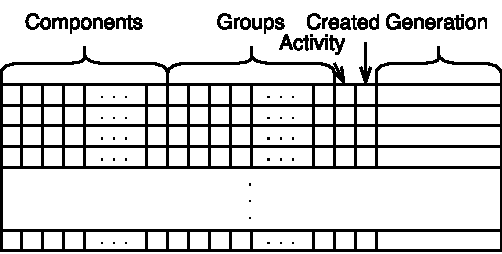
\includegraphics[width=\linewidth]{BAC-DES11}}
	\caption{Tabulka metadat, indexy jednotlivých entit jsou implicitní indexy řádků.}
	\label{Fig:DESMetadata}
\end{figure}

Důležitou součástí \emph{ECS} je možnost pracovat pouze s entitami, které mají požadované komponenty (\uv{aspekty}). Z tohoto důvodu je součástí zprávy entit i možnost filtrování (třída \textbf{EntityFilter}). Filtrovat lze pomocí seznamu požadovaných komponent, ale je také možno definovat zakázané komponenty, nebo specifikovat požadovanou úroveň aktivity entit (aktivní/neaktivní).

Poslední částí podsystému zprávy entit je třída \textbf{Entity}, jejíž funkcionalita zjednodušuje práci s \emph{ECS}. Operace na ní provedené jsou pouze přesměrovány na \textbf{Universe}, spolu s příslušným identifikátorem entity. Pomocí této třídy lze také \emph{ECS} propojit s okolním \emph{objektově orientovaným} kódem.

\begin{figure}[H]
	\tmpframe{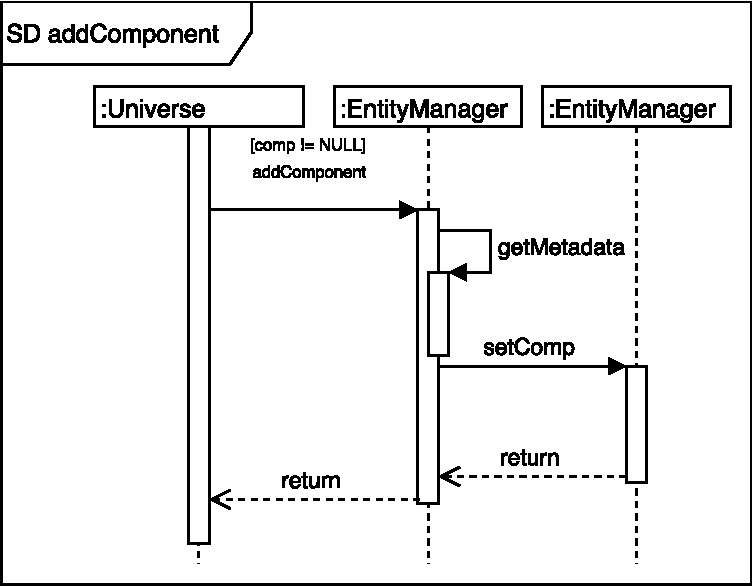
\includegraphics[width=\linewidth]{BAC-DES10}}
	\caption{Sekvenční diagram modifikace metadat při přidání komponenty, pokračování obr. \ref{Fig:DESAddComp}.}
	\label{Fig:DESAddEnt}
\end{figure}

Nevýhodou udržování informací o přítomnosti komponent na dvou místech je, že při každé změně je nutné, aby byla provedena i v metadatech. Příkladem tohoto problému je operace přidání komponenty, jejíž sekvenční diagram lze vidět na obr. \ref{Fig:DESAddComp}. Pokud je první fáze (přidání komponenty z pohledu \textbf{Component Manager}) úspěšná, je nutné upravit metadata.

\section{Systémy a skupiny}
\label{Chap:SysGroup}

\emph{Systém}, podle \emph{ECS} paradigmatu, obsahuje pravidla pro výběr vhodných entit a akce, které na nich provádí. Entity jsou filtrováni pomocí množiny požadovaných komponent (aspektů). Vstupem \emph{systému} je tedy seznam entit, které vyhovují filtračním pravidlům a jeho cílem je transformovat dané entity a jejich komponenty pomocí definované akce. Tato myšlenka je základem podsystémy zprávy \emph{systémů}. 

Předpokladem, při návrhu tohoto entitního systému je, že i přeš vysoký počet entit, které se v systému mohou nacházet v jeden okamžik, bude množství skutečně používaných entit \footnote{Těch, které budou používány jako součást některého ze systémů.} nižší. Z tohoto předpokladu vychází myšlenka \emph{skupin}, které jsou plní funkcí vyrovnávací paměti \emph{systémů}. \emph{Skupina} je množinou entit, které splňují požadavky specifikované filtrem. Oproti původnímu návrhu, kdy každý \emph{systém} iteruje (lineárně prochází) nad seznamem všech existujících entit v entitním systému, se při použití skupin již prochází pouze takové entity, které odpovídají požadavkům daného systému.

Jednou z nevýhodou použití \emph{skupin} je nutnost skupiny udržovat aktuální, čímž je pověřen podsystém zprávy \emph{skupin}. Díky potřebě udržování seznamu entitních identifikátorů způsobuje tento systém také vyšší použití paměti. Poslední důležitou vlastností je, že tato funkce předpokládá, že množina všech entit je větší, než množina používaných entit. Pokud tento předpoklad neplatí, potom není vhodné systém \emph{skupin} používat.

\begin{figure}[H]
	\tmpframe{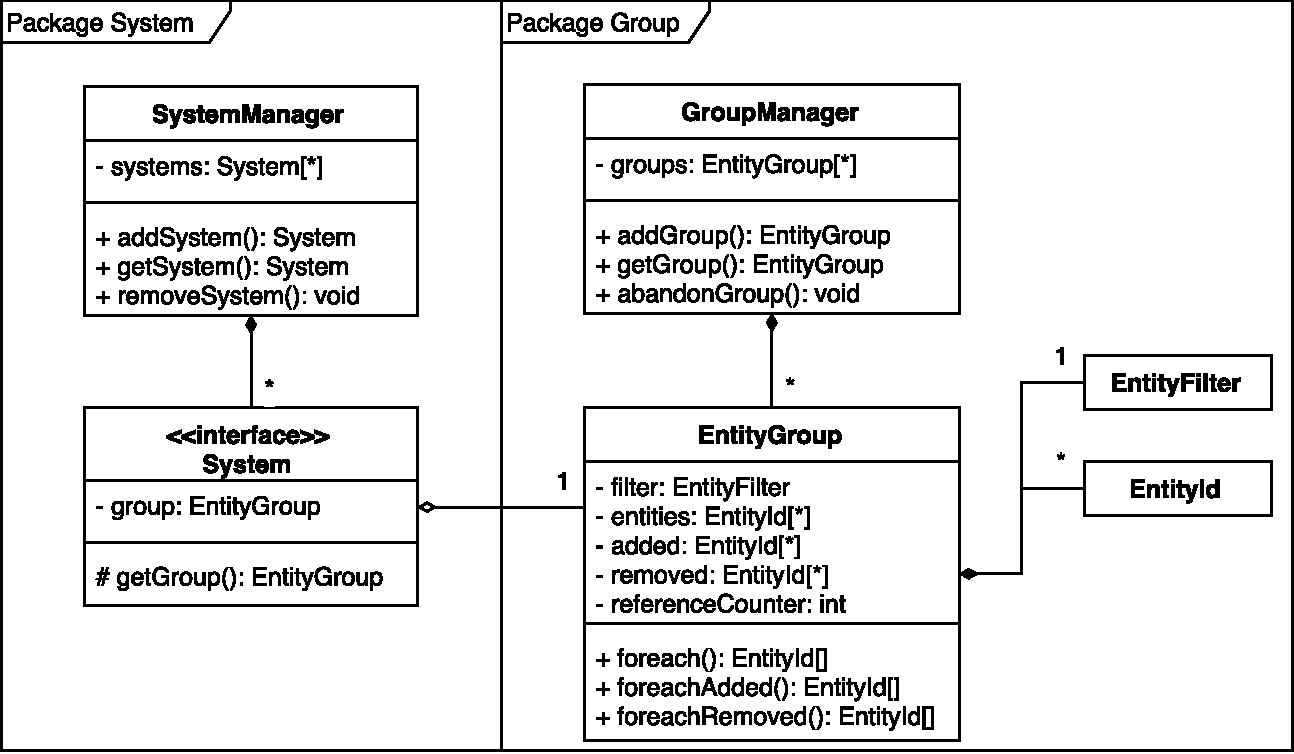
\includegraphics[width=\linewidth]{BAC-DES3}}
	\caption{Diagram tříd podsystému zprávy \emph{systémů}.}
	\label{Fig:DESSystemDiagram}
\end{figure}

Cílem podsystému zprávy \emph{systému} (obr. \ref{Fig:DESSystemDiagram}), je údržba systémů a jejich vazba na skupiny. Třída \textbf{SystemManager} umožňuje přidávání a odběr nových systémů. \emph{Systémy} jsou definovány uživatelem, ktery vytvoří vlastní třídu, která dědí ze základní třídy \textbf{System}. Dále uživatel musí specifikovat požadované vlastnosti entit -- vyžadované / zakázané komponenty a úroveň aktivity. Následně je možné nový typ \emph{systému} přidat pomocí manažerské třídy. 

\begin{figure}[H]
	\tmpframe{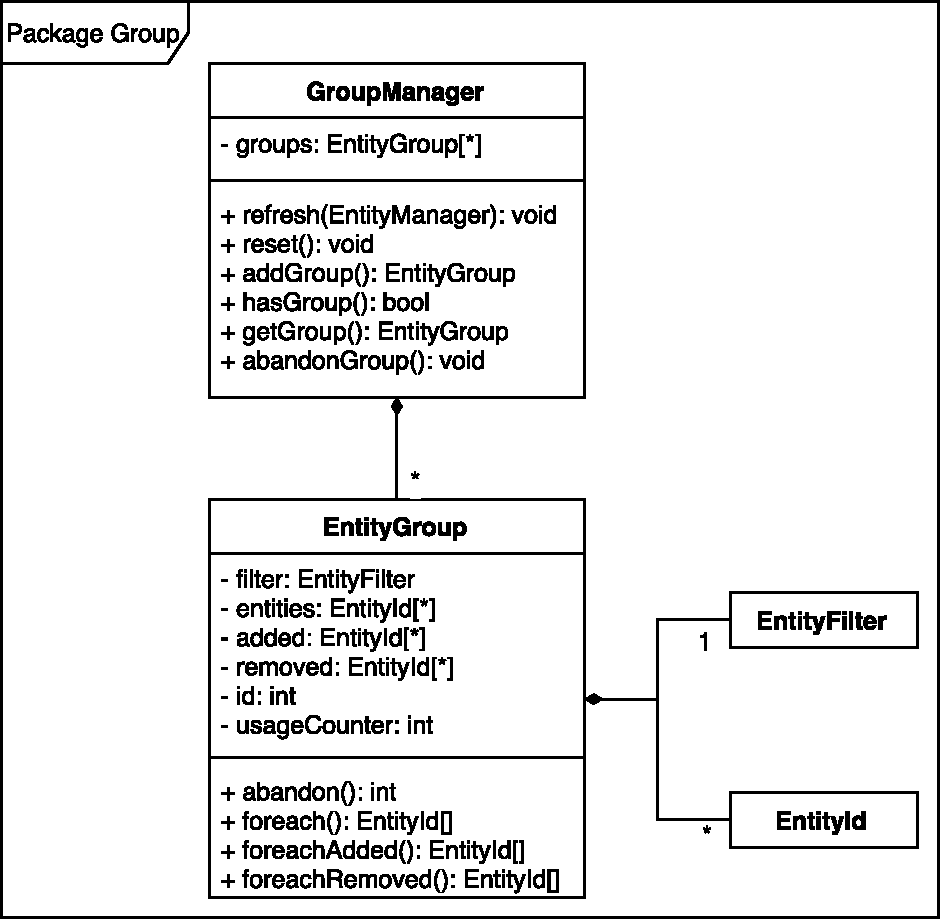
\includegraphics[width=\linewidth]{BAC-DES4}}
	\caption{Diagram tříd podsystému zprávy \emph{skupin}.}
	\label{Fig:DESGroupDiag}
\end{figure}

\emph{Skupiny} (\textbf{EntityGroup}) obsahují 3 seřazené seznamy entitních identifikátorů, jejich významy jsou následující -- přidané entity, odebrané entity a skutečný seznam všech vyhovujících entit. Důvod pro existenci prvních dvou je primárně umožnit uživateli propojit entitní systém se systémy okolními, které (např. fyzikální simulace) potřebují objekty registrovat.

Důležitou vlastnosti \emph{skupin} je možnost přidávat a odebírat je za běhu aplikace \footnote{Některé systémy nemusí zpracovávat entity po celý běh aplikace.}. Tato vlastnost je umožněna skrz podsystém zprávy \emph{skupin} (\ref{Fig:DESGroupDiag}). Každá \emph{skupina} obsahuje \uv{počítadlo referencí}, které reprezentuje na kolika různých místech je \emph{skupina} používána. V případě, že počítadlo dosáhne hodnoty 0, je \emph{skupina} odstraněna (nebo je pouze zastaven její běh). Zpráva \emph{skupin} závisí na entitních metadatech, které umožňují efektivnější aktualizace jejich obsahu \footnote{Více o tomto problému je součástí implementační části \ref{Chap:ImplSystem}.}.

\section{Paralelní přístup}

Díky modulárnímu návrhu entitního systému, který byl zatím předveden je implementace základních typů paralelního přístupu velmi přímočará. Mezi základní typy paralelizmu, který entitní systém podporuje jsou paralelizmus na úrovni entit a paralelizmus na úrovni systému.

Paralelizmus na úrovni entit využívá \emph{datového paralelizmu}, kde množina entit, nad kterou systém vykonává akce je rozdělena mezi požadovaný počet paralelních vláken. Tento typ paralelizmu je vhodný pouze v případech, kdy akce vykonávají transformace na entitách (a jejich komponentách), bez potřeby informací z ostatních entit. 

Paralelizmus na úrovni systémů lze přirovnat k \emph{úkolovému paralelizmu}, kde každé vlákno zpracovává rozdílný systém. Tento způsob má opět omezení -- systémy nemohou přistupovat ke stejným komponentám (stejných entit). Tyto dva způsoby paralelizmu lze kombinovat.

V situacích, kdy není možné použít ani jednu z těchto možností, nebo při manipulaci globálního kontextu z několika vláken, např. mazání entit, změna aktivity, je nutné použít jiné řešení. Jedním způsobem, jak tento problém vyřešit, je použití zámků (např. vzájemné vyloučení -- \uv{mutex}), které budou tyto metody chránit před problémy souběhu (\uv{race condition}). Zámky jsou čistým způsobem, jak implementovat bezpečný paralelizmus, ale vysokém počtu operací zamčení a odemčení je možné ztratit výkon, který byl získán paralelním zpracováním \footnote{Pokud jsou operace chráněné zámky používány často, je možné paralelní aplikaci redukovat na aplikaci sekvenční.}. Kvůli těmto nevýhodám je součástí návrhu také třetí metoda paralelizace -- pomocí \emph{množin změn}.

\emph{Množiny změn} umožňují jednotlivým vláknům odkládat provedení požadovaných operací na pozdější dobu, kdy již bude možné zaručit, že nedojde k problémům souběhu. Aktuální stav světa (entit, komponent apod.), pro každé vlákno, je vytvořen překrytím stavu globálního světa danou \emph{množinou změn}. Pokud vlákno použije operaci přidání komponenty, ke specifikované entitě, skutečné vykonání operace nad globálním kontextem bude odloženo, ale informace o této operaci bude přidána do \emph{množiny změn} aktuálního vlákna.

\begin{figure}[H]
	\tmpframe{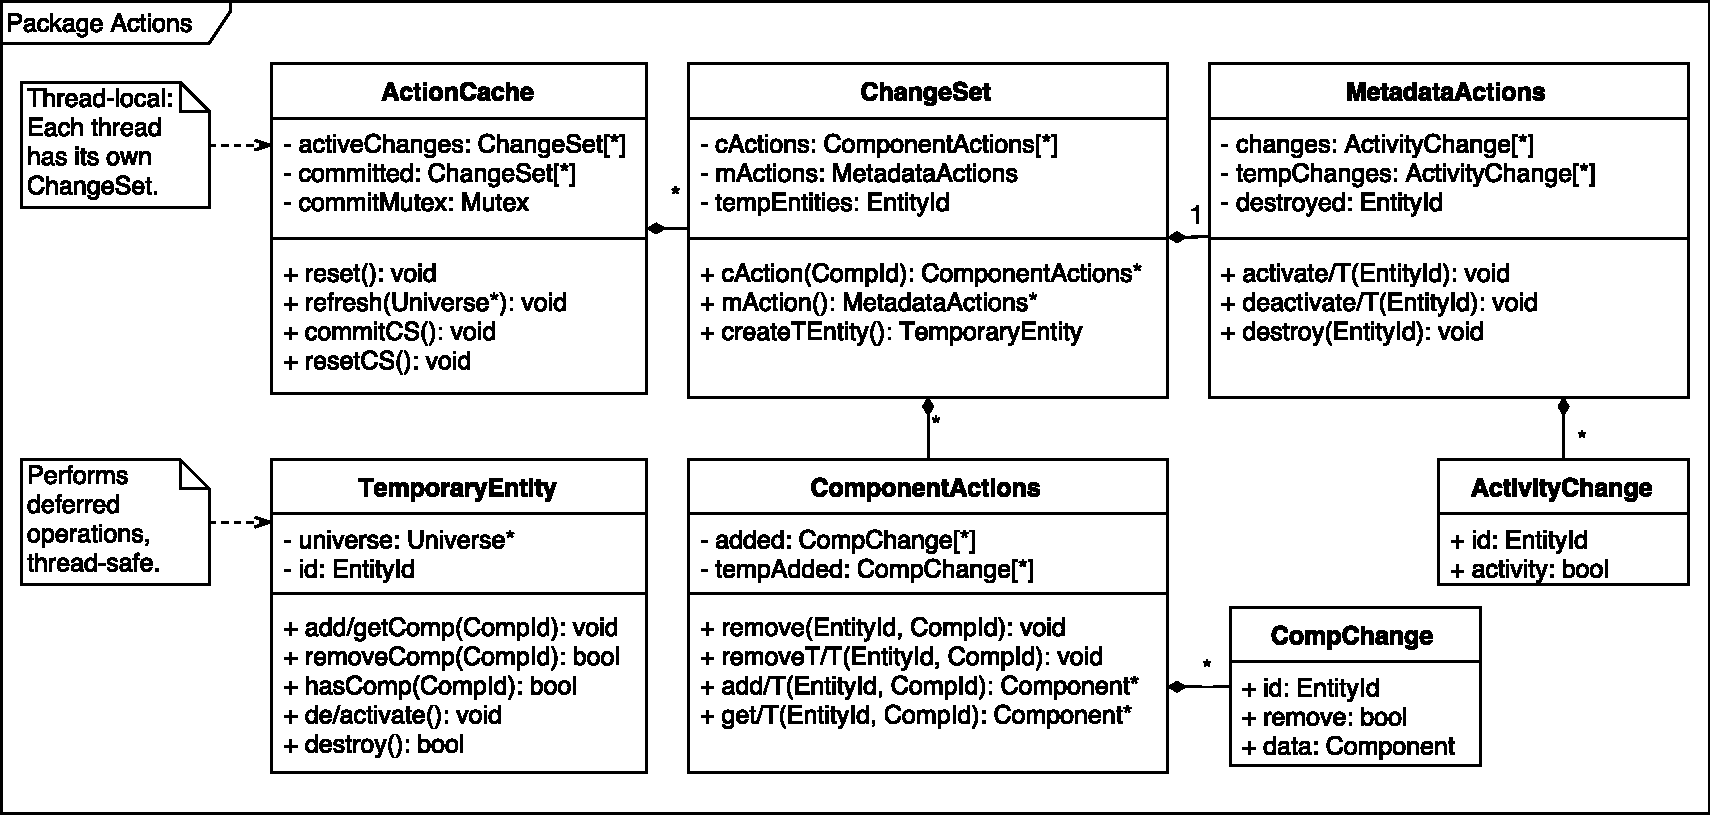
\includegraphics[width=\linewidth]{BAC-DES7}}
	\caption{Diagram tříd podsystému zprávy \emph{akcí}.}
	\label{Fig:DESActionDiag}
\end{figure}

Základem podsystému \emph{množin změn}, jehož diagram lze vidět na obr. \ref{Fig:DESActionDiag}, jsou třídy \textbf{ActionCache} a textbf{ChangeSet}. Úkolem \textbf{ActionCache} je zajistit přístup k instanci \emph{množin změn}, která bude pro každé vlákno unikátní. Dále umožňuje také potvrzení (\textbf{commitSC}), nebo zrušení (\textbf{resetCS}) \emph{množiny změn} aktuálního vlákna. 

Zajímavým problémem je odložená tvorba entit a následné provádění operací nad nimi. Pro operace, které jsou provedeny nad \emph{reálnými} entitami \footnote{Takové entity, které jsou již vytvořeny v globálním kontextu.} je možno specifikovat cílovou entitu pomocí jejího identifikátoru. Jedním možným řešením je zakázat provádění operací nad dočasnými entitami, nebo zrušit koncept dočasných entit kompletně a provádět operace vytvoření entity okamžitě \footnote{Toto by znamenalo použití zámků na celý podsystém zprávy entit a metadat.}. Druhým řešením, které je součástí tohoto návrhu, je přiřazení speciálního typu identifikátoru dočasným entitám, který bude později převeden na identifikátor reálné entity. Operace, jejíž provedení je odloženo na později, mají postfix \uv{\textbf{D}} (\uv{deferred}) a operace, které pracují s dočasnými entitami jsou zakončeny \uv{\textbf{T}} (\uv{temporary}).

\emph{Množiny změn} samotné jsou reprezentovány třídou \textbf{ChangeSet}, která obsahuje odložené \emph{akce}. \emph{Akce} je možno rozdělit na typy podle změn:
\begin{itemize}
	\item Změny metadat -- rušení entit, změna aktivity entit.
	\item Změny komponent -- přidání/odebrání komponent, změna hodnot komponent.
\end{itemize}
\noindent a podle cílové entity: 
\begin{itemize}
	\item Reálné entity -- operace obsahuje identifikátor reálné entity.
	\item Dočasné entity -- operace obsahuje identifikátor dočasné entity.
\end{itemize}

\section{Tok řízení}

Výše navržený entitní systém se vždy nachází v jedné z následujících fází -- \emph{inicializace}, \emph{iterace} nebo \emph{obnova}. Diagram řízení toku, který tyto fáze obsahuje, lze vidět na obr. \ref{Fig:DESFlow}.

\begin{figure}[H]
	\begin{center}
	\tmpframe{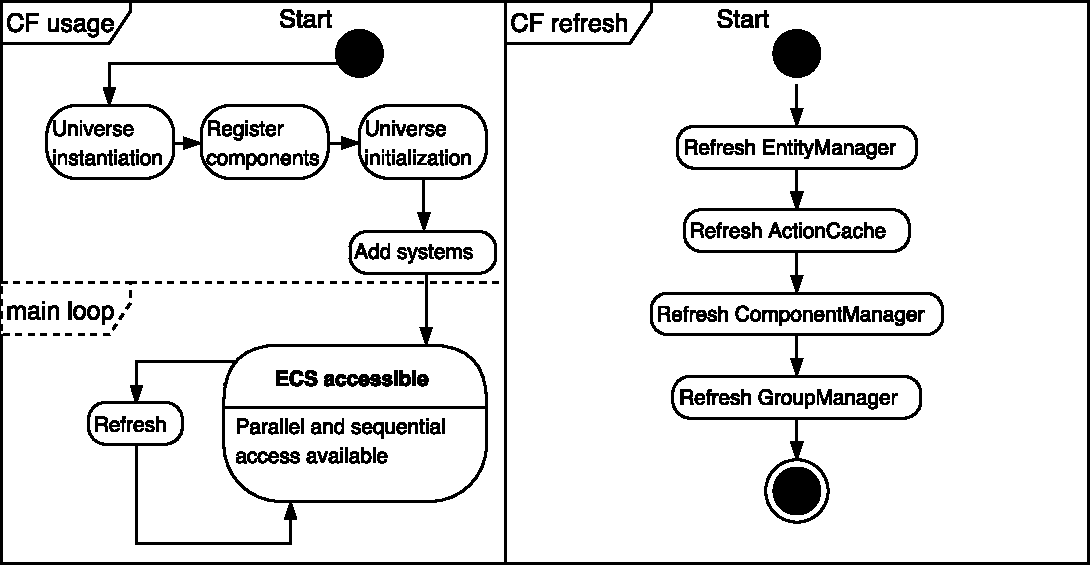
\includegraphics[width=0.9\linewidth]{BAC-DES9}}
	\end{center}
	\caption{Digram toku řízení komponentního systému.}
	\label{Fig:DESFlow}
\end{figure}

Prvním krokem ve fázi inicializace je konstrukce (vytvoření instance) třídy \textbf{Universe}, jejíž součástí je inicializace jednotlivých podsystémů. Potom je již možno registrovat typy komponent, které je potvrzeno závěrečnou inicializací objektu \textbf{Universe} \footnote{Po inicializaci již není možno přidávat nové typy komponent.}, čímž se entitní systém přesunuje do fáze \emph{iterace}. 

Fáze \emph{iterace} umožňuje plný přístup k entitnímu systému ze strany uživatele. Kromě práce s entitami a komponentami, je také možné přidávat a odebírat \emph{systémy} a \emph{skupiny}. Obsah jednotlivých \emph{skupin} je v této fázi konstantní, čímž je umožněna práce \emph{systémům}. V okamžiku, kdy již neběží žádné \emph{systémy} je možné přejít do fáze \emph{obnovy}, použitím operace \textbf{refresh}.

Úkolem \emph{obnovovací} fáze je posunutí entitního systému do následujícího stavu, ze stavu aktuálního a dokončení operací, které by vedly k porušení konzistence systému. Tohoto cíle je dosaženo postupným voláním operace \textbf{refresh} na jednotlivé podsystémy, jejichž pořadí lze vidět na obr. \ref{Fig:DESFlow}. Obnova entitního podsystému umožňuje dokončení operací přidání a odebrání \emph{skupin}, u kterých je nutné měnit počet sloupců v tabulce metadat. Následuje aplikace \emph{množin změn}, kdy jsou dokončeny odložené operace. Obnova pokračuje volání \textbf{refresh} nad jednotlivými nosiči komponent, kterým je tímto umožněna reorganizace dat. Poslední částí je příprava obsahu \emph{skupin} pro příští fázi \emph{iterace}. Po dokončení obnovy je systém opět uveden do fáze \emph{iterace}.

\chapter{Implementace}
\todo{Shrnutí návrhu}
\blind[2]

\section{Použité knihovny a přenositelnost}
\todo{zduvodneni pouziti c++ Zdůvodnění nepoužití knihoven. C++14, Linux, Windows. Header-only}
\blind[2]

\section{Komponenty}
\todo{Rekapitulace vlastností, které komponenta musi splnit. Registrace, generování identifikátorů. Uživatelské nosiče}
\blind[3]

Jelikož je metoda \textbf{getHolder} volána při každé operaci, která pracuje s komponenty, mělo by být mapování mezi typem komponent a jejich nosiči (skrz registr komponent) implementováno

\section{Správa entit}
\todo{Potřebné informace, implementace, datové struktury, optimalizace}
\blind[3]
identifikátor dočasných entit

\section{Systémy a skupiny}
\label{Chap:ImplSystem}
\todo{Super třída, filtry, přístup - iterace. Přidání systému, volitelná skupina - added/removed.}
\blind[3]

Vime, ktere akce na entitach probihaji
3-way merge group

\section{Podpora paralelizmu}
\todo{2 způsoby paralelizmu - dělení skupin, change-sety}
\blind[3]

\section{Obnovovací fáze}
\todo{Pořadí refresh. Obnovení aktuality skupin.}
\blind[2]

\chapter{Použití knihovny}

\section{Demo hra}
\todo{Popis principů hry}
\blind[1]

\section{Návrh}
\todo{Komponentní návrh}
\blind[3]

\section{Zhodnocení}
\todo{Výkon, návrh, jednoduchost}
\blind[3]


\chapter{Vyhodnocení}
\todo{Shrnutí, popis co bude v této kapitole}
\blind[1]

\section{Testování knihovny}
\todo{Unit testing, benchmarky}
\blind[2]

\section{Testované sestavy}
\todo{Hardware sestavy - PC, notebook. Tabulka identifikace}
\blind[1]

\section{Výkonnostní testy}
\todo{Výkon při různých zatíženích - procenta přidaných/odebraných. Grafy.}
\blind[1]
\todo{Porovnání nosičů komponent. Grafy.}
\blind[1]
\todo{Seriové vs paralelní - počet vláken. Grafy.}
\blind[1]

\section{Porovnání}
\todo{Výkonostní porovnání oproti jiným ECS knihovnám, Unity? Grafy.}
\blind[2]

\subsection{Implementace}
\todo{Použité knihovny, základní popis implementace}
\blind[2]

\subsection{Výsledek}
\todo{Poznatky a výsledky získané ze hry. Grafy?}
\blind[2]


\chapter{Závěr}
\todo{Využití komponentních systémů a aktuální stav} 
\blind[1]
\todo{Návrh, prototypy, priority} 
\blind[1]
\todo{Implementace, rozšiřitelnost, přenositelnost}
\blind[1]
\todo{Experimenty, srovnání, demo hra}
\blind[1]
\todo{Možnosti rozšíření}
\blind[1]
dynamicke komponenty za behu

%\begin{figure}
%	\tmpframe{
\includegraphics[width=\linewidth]{TODO-image}}
%	\caption{Obrazek \todo{Obrazek}}
%\end{figure}

%=========================================================================
